\documentclass[preprint,12pt]{elsarticle}
\usepackage{lmodern}
\ifdefined\pdfgentounicode
  \input{glyphtounicode}
  \pdfgentounicode=1
\fi
\usepackage{amsmath,amssymb,amsfonts,mathtools,amsthm,bm}
\usepackage{booktabs,graphicx,array,tabularx,placeins,float,url}
\usepackage[hidelinks]{hyperref}
\hypersetup{pdfauthor={Ali Eslami and Jiangbo Yu}}
\usepackage[protrusion=true,expansion=false]{microtype}
\graphicspath{{figures/}{./}}
\allowdisplaybreaks
\setlength{\emergencystretch}{3em}
\interdisplaylinepenalty=2500
\newtheorem{assumption}{Assumption}
\newtheorem{theorem}{Theorem}
\newtheorem{proposition}{Proposition}
\newtheorem{corollary}{Corollary}
\newtheorem{remark}{Remark}
\newtheorem{definition}{Definition}
\newcommand{\R}{\mathbb{R}}
% elsarticle includes the word ``Appendix'' in appendix-section references.
\newcommand{\appref}[1]{\ref{#1}}
\journal{Transportation Research Part B: Methodological}



\begin{document}
\begin{frontmatter}
\title{Formal Guarantees for Trustworthy Agent-Mediated Urban Perimeter Control}
\author[mcgill]{Ali Eslami}
\ead{ali.eslami@mcgill.ca}
\author[mcgill]{Jiangbo Yu\corref{cor1}}
\ead{jiangbo.yu@mcgill.ca}
\cortext[cor1]{Corresponding author.}
\affiliation[mcgill]{organization={Department of Civil Engineering, McGill University},
 addressline={817 Sherbrooke Street West}, city={Montreal}, state={Quebec},
 postcode={H3A 0G4}, country={Canada}}
\begin{abstract}\fontsize{11}{13}\selectfont
Urban perimeter control must manage regional congestion and boundary queues
while satisfying time-specific service obligations. AI agents can support
traffic operators by interpreting evolving network conditions, incidents,
and service priorities and translating them into adaptive control and
replanning requests. However, each new agent-proposed plan must remain
compatible with the evolving traffic state, uncertainty, and outstanding
service obligations. We therefore formulate a runtime certification problem
for agent-proposed perimeter-control plans and develop a
transportation-specific framework that provides formal guarantees of
physical and service feasibility before execution. The framework checks
whether a proposed plan respects vehicle conservation, nonnegative traffic
states, boundary-storage limits, and service deadlines under uncertainty. It
then decides whether the plan can be executed as proposed, should be
modified to restore feasibility, or should be rejected while the previously
accepted plan remains in use, and, when the terminal conditions are
certified, ensures that accepted plans end in a state from which feasible
operation can continue. Numerical studies show that the certificate leaves
feasible plans unchanged, traffic-specific structure reduces conservatism,
and checked repair recovers feasible alternatives. Further experiments show
that the framework can accept beneficial changes while rejecting requests
that would violate boundary-storage or service constraints, including under
computation delays and agent-context errors. Overall, the framework advances
trustworthy AI for transportation systems by providing formal guarantees
that connect adaptive agent decisions to physically and operationally
feasible traffic control.
\end{abstract}
\begin{keyword}
Agentic AI \sep Macroscopic fundamental diagram \sep Perimeter control \sep Runtime certification \sep Model predictive control
\end{keyword}
\end{frontmatter}

\section{Introduction}
\label{sec:new-introduction}

Urban perimeter control regulates flows into and between regions as
congestion and external arrivals change. Regional accumulation affects
network traffic production through the macroscopic fundamental diagram
(MFD), which provides a tractable network-scale description of congestion
and trip completion
\cite{daganzo2007gridlock,geroliminis2008existence,daganzo2008analytical,geroliminis2011properties,leclercq2014cross}.
From an operator's perspective, the problem is to regulate regional
accumulation, manage vehicles waiting at region boundaries, and satisfy
time-specific service obligations. These requirements become more difficult
to coordinate when incidents, demand conditions, or operating priorities
change during execution.

Classical MFD perimeter-control methods address regional congestion through
feedback gating and multivariable boundary-flow control
\cite{keyvan2012gating,aboudolas2013perimeter}. Stability analysis and
control-Lyapunov-function designs establish regulation properties under
prescribed traffic dynamics \cite{haddad2012stability,zhong2018robust},
while robust, hybrid, and adaptive formulations extend perimeter regulation
to uncertain observations, switching actions, and changing operating
conditions
\cite{mohajerpoor2020hinf,hajiahmadi2015hybrid,haddad2020adaptive,kouvelas2017adaptive}.

Predictive perimeter control optimizes sequences of gate commands over an
MFD model \cite{geroliminis2013mpc}. Multi-region formulations account for
spatial heterogeneity and route guidance
\cite{ramezani2015heterogeneity,sirmatel2018economic}, while exterior queues
and cordon storage capture the waiting cost and spillback created by
metering \cite{haddad2017queues,ni2019cordon}. State and demand estimation
further support predictive operation when traffic conditions must be
reconstructed from measurements \cite{sirmatel2019estimation}, and recent
MFD calibration work explicitly characterizes loading--recovery variation
and uncertainty \cite{ma2025mfduq}.

AI-based decision tools provide an additional way to adapt perimeter control
as traffic conditions and operator objectives change. Data-driven
perimeter-control methods have used adaptive dynamic programming and
reinforcement learning to learn gating policies from traffic experience
\cite{chen2022dataefficient,chen2024iadp}, while multi-agent approaches
coordinate regional metering, heterogeneous cordon gates, and decentralized
control \cite{zhou2023scalable,yu2025physicsperimeter,li2024beyond}. Related
traffic-signal and language-model studies show how AI systems can generate
actions, interpret contextual information, coordinate decisions, and invoke
external tools
\cite{wei2019presslight,wei2019colight,llmlight2023,masri2025llmtraffic,collmlight2025,trafficgpt2024,openti2024,virtualpolice2026,yu2025statespace}.

These capabilities can support traffic operators when changing network
conditions or service priorities require new control decisions. In this
work, an AI agent serves this higher-level role: it interprets evolving
operating priorities and invokes computational tools, such as numerical
planners, to generate candidate perimeter-control plans.

This added flexibility creates a certification requirement whenever a
proposed plan replaces the plan currently in operation. Each agent-proposed
plan must remain compatible with the traffic state at the time of
activation, uncertainty in that state and future arrivals, available
boundary storage, and any service obligations that are still active.
Evaluation of a newly proposed plan therefore incorporates the traffic state
and outstanding obligations inherited from the operation already under way.
The operator needs a principled way to decide whether the new plan may
replace the current one, whether it should be modified, or whether the
previously accepted plan should remain in operation.

Runtime assurance provides a natural foundation for this decision. Simplex
architectures retain a verified fallback controller
\cite{simplex,mehmood2022black}; control barrier functions and shielding
restrict unsafe actions \cite{ames2017,alshiekh2018}; predictive safety
filters evaluate future constraint satisfaction
\cite{wabersich2021,hsu2023safety}; and runtime-assurance and
reference-governor methods formalize the transfer of control authority
\cite{fisac2019,hobbs2023runtime,gilbert2002generalized,garone2017reference}.
Reachability methods additionally provide tools for propagating uncertainty
over future trajectories \cite{coogan2020mixed,kochdumper2021sparse}. These
methods establish foundations for supervising learning-enabled decisions.
Urban perimeter control also provides structure that can be exploited
directly: vehicles wait at region boundaries for admission to particular
destinations, regional inventories and boundary queues are physically
coupled, and service requirements may remain active across successive
planning requests.

We use this transportation structure to construct a runtime certificate for
agent-proposed perimeter-control plans. The certificate checks whether a
candidate plan satisfies vehicle conservation, nonnegative traffic states,
boundary-storage limits, and time-specific service requirements for all
states and arrivals represented by the uncertainty model. A key observation
is that a vehicle waiting for admission to a destination and the
corresponding destination inventory form a conserved quantity with respect
to that admission flow. Combining these quantities therefore removes the
admission decision from part of the uncertainty propagation. Positivity,
independent queue bounds, and signed uncertainty representations further
tighten the resulting bounds while preserving dependencies in the uncertain
traffic state. Together, these ingredients provide a transportation-specific
representation for checking regional inventories, queues, control inputs,
and service constraints over the planning horizon.

The certificate is then integrated with sequential planning and execution.
If a proposed plan satisfies the required conditions, it can replace the
currently active plan with its commands preserved. A rejected plan enters a
checked repair procedure that searches for a nearby feasible alternative,
with every repaired candidate returned to the same certificate before
execution. If no replacement is accepted, the previously accepted plan
remains active through its certified validity interval. When the terminal
conditions are certified, the framework ensures that accepted plans end in a
state from which feasible operation can continue. It also accounts for
traffic evolution while a new plan is being computed and certified.

The resulting framework provides a formal interface between adaptive
AI-based planning and physical traffic execution. The interface determines
when plans produced by AI models and computational tools are admissible for
the transportation system. The numerical evaluation examines certification
conservatism and checked repair. Further experiments show that the framework
can accept beneficial changes while rejecting requests that would violate
boundary-storage or service constraints, including under computation delays
and agent-context errors.

The paper makes four main contributions:
\begin{enumerate}
\item We define the requirements that agent-proposed perimeter-control plans
must satisfy before execution. These requirements connect operator requests
to numerical planning tools and ensure that each new plan accounts for the
current traffic state, uncertainty, existing service obligations, and plan
timing.

\item We develop a traffic-specific method for checking physical constraints
and service deadlines under uncertainty. The method uses vehicle
conservation, nonnegative vehicle counts, and the links between boundary
queues and regional traffic to obtain tighter bounds on future traffic
states. It retains relationships between uncertain traffic quantities and
extends to networks with several entry queues.

\item We prove guarantees for accepting, repairing, and rejecting proposed
plans. Plans that pass certification can be executed unchanged. With a
backup certified for the same traffic information and requirements, a
completed repair search selects the certified plan closest to the proposed
plan within a predefined finite set, measuring the difference through their
planned control actions. If a proposal is rejected or computation runs out
of time, the previously accepted plan remains in use through its certified
validity interval. When the required terminal conditions are also certified,
feasible operation can continue beyond plan expiry.

\item We provide reusable test cases involving regional congestion, boundary
queues, and service deadlines. Numerical studies examine the tightness of
the certification bounds and how well repair recovers feasible plans.
Further experiments test successive plan changes, networks with several
regions, computation delays, and errors in the information given to the
agent.
\end{enumerate}

Section~\ref{sec:new-problem} formulates the traffic-control problem. Section~\ref{sec:new-agent} defines the agent and planning interface, and Section~\ref{sec:new-certification} develops plan certification and execution. Section~\ref{sec:new-evidence} evaluates the method; Section~\ref{sec:new-discussion} discusses operational implications. Detailed proofs and numerical specifications appear in the appendices and supplement.

\begin{table}[!t]
\centering\small
\caption{Notations used throughout the paper. Traffic inventories are expressed in units of
100 vehicles unless a table states physical vehicles.}
\label{tab:nomenclature}
\renewcommand{\arraystretch}{0.98}
\begin{tabular}{@{}p{0.20\linewidth}p{0.72\linewidth}@{}}
\toprule
Symbol & Meaning\\
\midrule
$n_i$, $n_{ij}$ & Regional accumulation; vehicles in region $i$ destined for $j$\\
$z$, $x$, $M$ & Exterior waiting inventory; physical state; total vehicle inventory\\
$u_{ij}$, $a$ & Fractional gate command; realized exterior admission flow\\
$\Lambda$, $d^{\rm int}_{ij}$ & Exterior arrivals; destination-specific internal demand\\
$d$, $\bar w_{\rm veh}$ & Sensing half-width (vehicles); physical arrival-residual bound (veh/h)\\
$\bar w_x$ & Normalized arrival-residual bound $\bar w_{\rm veh}/100$ (inventory units/h)\\
$\mathcal S_t$ & Decision record: state set, uncertainty, task, active plan, time and versions\\
$P$, $P^B$, $\mu_B$ & Proposed plan; verified continuation; terminal backup policy\\
$P_a$, $c$ & Destination-allocation matrix; network destination-class vector\\
$t_f$, $\eta$ & Example service deadline and inventory limit\\
$T_r$, $g_r$, $\eta_r$ & General service time, row vector and threshold\\
$\theta_i$, $\lambda_{\rm rep}$ & Agent task record; predictive-repair interpolation weight\\
$K_b$, $K$, $\mathcal K$ & Feedback gain; local block count; terminal invariant set\\
$\beta_j^{\rm phys}$, $b_a$ & Physical constraint-row limit; admission-incidence vector\\
$y$, $L$ & Conservation-coordinate state and its invertible transform\\
$r_l$, $R_l$ & Starting and trial-tube radii on interval $l$\\
$a_{il}$, $b_{ijl}$ & Local diagonal and off-diagonal Jacobian bounds\\
$\xi$, $\Gamma_l$, $\zeta_l$ & Initial uncertainty, signed generator and nonlinear remainder\\
$z_e$ & Prediction-error coordinate used only in the enclosure proof\\
$J_R$, $J_Q$, $J_D$ & Native regulation, queue-economic and weighted-priority objectives\\
$p$, $E$, $x^R$ & Regional-priority weight; finite-plan endpoint; native four-state vector\\
$\mathcal C$, $\mathcal F_{\mathcal C}$, $\widehat{\mathcal F}_{\mathcal C}$ & Planning contract; robust feasible and checker-certified plan sets\\
$X_i^A$, $h_i$, $\iota_i$ & Agent interface state, memory and supplied contextual view\\
$B_\omega$ & Fraction of requested priority benefit recovered by repair\\
$\mathrm{TTS}$ & Total time spent, including exterior waiting; vehicle-hours (veh-h)\\
\bottomrule
\end{tabular}
\end{table}

\FloatBarrier
\section{Two-Region MFD Perimeter-Control Problem}
\label{sec:new-problem}
Here, we use a two-region network as the primary setting because it is the smallest
configuration that captures interregional transfers, destination-specific
vehicle classes, exterior admission, and regional service requirements while
keeping the certification construction transparent. The model also follows
established two-region MFD perimeter-control formulations. Section~\ref{sec:network-extension}
extends the certification construction to networks with multiple regions and
exterior queues.


\subsection{Traffic inventories, destination flows and boundary storage}

The physical state comprises the total vehicle accumulation in each region, destination-specific vehicle classes, and an exterior staging reservoir:
\begin{equation}
\begin{aligned}
x&=(n_1,n_2,n_{11},n_{22},n_{10},n_{20},z)^\top,\\
u&=(u_{12},u_{21},u_{02},u_{20})^\top.
\end{aligned}
\label{eq:new-state}
\end{equation}
Here $n_i$ denotes the total vehicle accumulation in region $i$, with
$i\in\{1,2\}$. The variable $n_{ij}$ counts vehicles currently in region
$i$ whose destination is $j$, where $j\in\{0,1,2\}$ and $j=0$ denotes the
exterior. Thus, $n_{ii}$ represents vehicles that complete their trips
within region $i$, $n_{12}$ and $n_{21}$ represent interregional traffic,
and $n_{10}$ and $n_{20}$ represent vehicles destined for the exterior.

Exterior-destined vehicles in Region~1 leave the network through Region~2.
Because the destination classes within each region sum to the regional total,
the interregional class inventories are recovered from the regional totals
and stored classes as
\[
n_{12}=n_1-n_{11}-n_{10}, \qquad
n_{21}=n_2-n_{22}-n_{20}.
\]
The separate queue $z$ represents vehicles waiting outside the controlled
regions for admission. One state unit represents 100 vehicles, and time is
measured in hours. Inventories are continuous aggregate quantities, and
their evolution is described by continuous-time differential equations.
The variables $n_{ij}$ describe stored vehicle inventories, and $q_{ij}$ below
describes their potential outflow rate in inventory units/h.

Following the two-region perimeter-control models in
\cite{zhong2018robust,geroliminis2013mpc}, we use the cubic MFD
\begin{equation}
\begin{aligned}
G(n)&=0.0014877n^3-0.29815n^2+15.0912n,\\
q_{ij}&=n_{ij}v(n_i),
\end{aligned}
\label{eq:new-mfd}
\end{equation}
where
$v(n)=0.0014877n^2-0.29815n+15.0912$
equals $G(n)/n$ for $n>0$ and is defined by continuity at $n=0$. The potential class outflow $q_{ij}$ is defined
before gating. The aggregate rate $G(n_i)$ describes potential trip
completion and transfer out of region $i$, allocated among destination
classes in proportion to their inventories. This MFD has a critical accumulation of 3391.93 vehicles
and a peak potential outflow of 22,691 veh/h. We impose an operational upper bound of 10,000 vehicles per region. This bound is a model constraint at which the fitted MFD retains positive production. Class flows assume comparable within-region trip
lengths, destination-proportional mixing, and adequate receiving supply
throughout the verified domain.

Exterior arrivals are $\Lambda(t)=\widehat\Lambda(t)+w(t)$, with specified
forecast $\widehat\Lambda$ and bounded measurable residual $w$.
For destination fraction $\pi=1/2$ toward Region~1,
\begin{equation}
a(z,u_{02})=\min\{60z,120u_{02}\},\qquad
\dot z=\Lambda-a.
\label{eq:new-admission}
\end{equation}
These branches represent a one-minute staging release time and commanded
admission capacity. The queue explicitly accounts for boundary storage
\cite{haddad2017queues}. Its limit measures aggregate overflow. Spatial
spillback requires a receiving-supply extension.

The gate commands are dimensionless fractions. Interregional and exit
commands multiply the corresponding potential class flows. Thus $u_{ij}=1$
permits the full potential flow and $u_{ij}=0$ blocks it. Exterior
admission instead follows \eqref{eq:new-admission}, with $u_{02}$ scaling
the admission capacity. Commands may vary over time or be held on finite
planning blocks. They represent aggregate boundary-flow allocations.
For a class with potential flow $q$ and associated gate fraction $u_g$,
the physical number transferred over $[t_a,t_b]$ is
$100\int_{t_a}^{t_b}u_g(t)q(t)\,dt$.

With fixed primitive demands and sums
$d^{\rm int}_1=d^{\rm int}_{11}+d^{\rm int}_{12}+d^{\rm int}_{10}$, $d^{\rm int}_2=d^{\rm int}_{22}+d^{\rm int}_{21}+d^{\rm int}_{20}$, conservation gives
\begin{equation}
\begin{aligned}
\dot n_1&=-q_{11}-(q_{12}+q_{10})u_{12}+q_{21}u_{21}+d^{\rm int}_1,\\
\dot n_2&=-q_{22}+(q_{12}+q_{10})u_{12}-q_{21}u_{21}
                 +a-q_{20}u_{20}+d^{\rm int}_2,\\
\dot n_{11}&=-q_{11}+q_{21}u_{21}+d^{\rm int}_{11},\\
\dot n_{22}&=-q_{22}+q_{12}u_{12}+(1-\pi)a+d^{\rm int}_{22},\\
\dot n_{10}&=-q_{10}u_{12}+d^{\rm int}_{10},\\
\dot n_{20}&=-q_{20}u_{20}+q_{10}u_{12}+d^{\rm int}_{20},\\
\dot z&=\widehat\Lambda+w-a.
\end{aligned}
\label{eq:new-plant}
\end{equation}
A transfer preserves a vehicle's destination while changing its current
region. For example, a vehicle transferred from class $n_{21}$ enters
$n_{11}$, which is already included in $n_1$. Its trip subsequently
completes at the local outflow rate $q_{11}$. Command changes preserve
physical inventories, which remain continuous across planning blocks.
The gate fractions satisfy
\begin{equation}
\mathcal U=\{u:0\le u\le1,\ |u_{21}-u_{12}|\le0.75,
\ |u_{20}-u_{02}|\le0.75\}.
\label{eq:new-gates}
\end{equation}
The six classes are nonnegative, $0\le n_1,n_2\le100$, and $0\le z\le20$.
Together with \eqref{eq:new-gates}, these give 24 affine state--command
inequalities, checked directly using the plan commands and unmodified
inventory values.
The initial state is $(30,30,15,15,5,5,2)$ and base exterior arrivals are
6000 veh/h. Internal demands are constructed once from this operating
record and held fixed across targets and policies
(\appref{app:new-model}).

\subsection{Service obligations and queue-inclusive performance}

The operator specifies service through scheduled affine rows
$g^\top x(t_f)\le\eta$, which can express a regional clearance target or an
imbalance band. For example, the original incident grid uses
\begin{equation}
100n_1(t_f)\le2850\ \text{vehicles},\qquad t_f=1\ \text{h}.
\label{eq:new-service}
\end{equation}
This requirement must hold at the specified deadline \(t_f\), even if the regional accumulation falls below the target earlier. The planner may change its control reference or soft optimization objective, but the authorized service target and its deadline can be changed only by the operator. The binding-service experiment uses 1700 vehicles
at the same deadline.

The planner minimizes queue-inclusive total time spent (TTS). Adding the regional and exterior-queue balances cancels internal transfers and admission flows, so the total inventory changes only through external arrivals, internal demand, and completed departures:
\begin{equation}
\begin{aligned}
M&=n_1+n_2+z,\\
\dot M&=d^{\rm int}_1+d^{\rm int}_2+\Lambda-F_{\rm out},\\
F_{\rm out}&=q_{11}+q_{22}+q_{20}u_{20},\\
\mathrm{TTS}&=100\int_0^{T_{\rm eval}} M(t)\,dt.
\end{aligned}
\label{eq:new-conservation}
\end{equation}
Here $T_{\rm eval}$ denotes the evaluation horizon. Queue time
$100\int_0^{T_{\rm eval}} z\,dt$ is already included. Completed departures
$100\int_0^{T_{\rm eval}} F_{\rm out}\,dt$ differ from potential MFD outflow,
which also counts transfers before gating. For matched arrivals and initial
inventory, departure differences equal
$-100\Delta M(T_{\rm eval})$. Including the exterior queue in TTS accounts for the time vehicles spend
waiting when admission is restricted.

\subsection{A reusable family of perimeter-control tasks}
\label{sec:benchmark-formulation}

We distinguish three tasks according to the transportation decision being
evaluated. Each task fixes the dynamics, available information, command limits,
initial condition and evaluation interval before comparing methods.

\paragraph{R: regional regulation}
The native two-gate formulation of \cite{zhong2018robust} uses four
destination classes $x^R=(n_{11},n_{12},n_{21},n_{22})^\top$ and regional
totals $n_1=n_{11}+n_{12}$, $n_2=n_{21}+n_{22}$. With the class flows in
\eqref{eq:new-mfd}, its balances are
\begin{equation}
\begin{aligned}
\dot n_{11}&=d^{\rm int}_{11}-q_{11}+u_{21}q_{21},\\
\dot n_{12}&=d^{\rm int}_{12}-u_{12}q_{12},\\
\dot n_{21}&=d^{\rm int}_{21}-u_{21}q_{21},\\
\dot n_{22}&=d^{\rm int}_{22}-q_{22}+u_{12}q_{12}.
\end{aligned}
\label{eq:benchmark-native}
\end{equation}
The task regulates both totals to $n_i^\star=30$ while maintaining
nonnegative classes, regional storage and the specified two-gate intervals.
We evaluate
\begin{equation}
J_R=10^4\int_0^{3/2}\bigl[(n_1-30)^2+(n_2-30)^2\bigr]\,dt.
\label{eq:benchmark-regulation-cost}
\end{equation}
Its units are veh$^2$-h. This native regulation task supplies a direct
comparison with the reproduced almost-smooth CLF law. The queue-aware tasks
below additionally require the admission and exit channels of
\eqref{eq:new-plant}.

\paragraph{Q: queue-inclusive economic planning}
At $t_0=1/3$ h, use the seven-state information set $\mathcal I_{t_0}$,
arrival forecast and bounded residual of \eqref{eq:new-plant}. A numerical
planner requests two constant gate blocks through the absolute endpoint
$E=1$ h. Subject to the physical rows, the objective is
\begin{equation}
J_Q(P)=100\int_{t_0}^{E}(n_1+n_2+z)\,dt.
\label{eq:benchmark-queue-cost}
\end{equation}
Exterior arrivals continue to join the queue when admission is restricted.
Thus $J_Q$ measures the traffic consequence of metering, including waiting
outside the controlled regions \cite{haddad2017queues}. The predictive tool
follows the MFD planning approach of \cite{geroliminis2013mpc} with the
explicit model, blocking and objective supplied here.

\paragraph{D: deadline-constrained plan replacement}
The same plant and information are supplemented by
$100n_1(E)\le\eta$ vehicles and a soft Region-2 priority with weight
$p\ge1$. The requested objective is
\begin{equation}
J_D(P)=100\int_{t_0}^{E}(n_1+p n_2+z)\,dt.
\label{eq:benchmark-priority-cost}
\end{equation}
For a physical sensing half-width $d$ vehicles and arrival-residual bound
$\bar w_{\rm veh}$ veh/h, define the normalized bound
$\bar w_x=\bar w_{\rm veh}/100$ in inventory units/h. The uncertainty
contract is
\begin{equation}
\begin{aligned}
\mathcal I_{t_0}&=\widehat x_{t_0}+[-d/100,d/100]^7,\\
|w(t)|&\le\bar w_x,\qquad t\in[t_0,E].
\end{aligned}
\label{eq:benchmark-contract}
\end{equation}
\paragraph{Feasible plans and certifiable plans}
For Tasks Q and D, collect the information set, uncertainty family, model,
physical rows, scheduled service rows and absolute interval $[t_0,E]$ in a
contract $\mathcal C$. The plan class consists of the executable finite
schedules defined in Section~\ref{sec:new-agent}. Write
$x_P(s;x_0,w)$ for their traffic trajectories. The robust feasible set is
\begin{equation}
\begin{aligned}
\mathcal F_{\mathcal C}=\{P:\;&\forall x_0\in\mathcal I_{t_0},\ w\in\mathcal W,\\
&H_jx_P(s;x_0,w)+J_ju_P(s;x_0,w)
                         \le\beta_j^{\rm phys}\\
&\hspace{1em}\text{for all }s\in[t_0,E]\text{ and physical rows }j;\\
&g_r^\top x_P(T_r;x_0,w)\le\eta_r
\quad\text{for all service rows }r\}.
\end{aligned}
\label{eq:benchmark-feasible-set}
\end{equation}
Here $\mathcal W$ contains all measurable residuals satisfying the stated
bound, and each service time $T_r$ lies in $[t_0,E]$. Membership also
requires a well-defined trajectory throughout that interval. Task Q has
an empty service-row collection. Task D includes the minute-60 regional
row. The checker identifies a computable subset of plans that satisfy these
requirements for every allowed initial state and arrival residual:
\begin{equation}
\widehat{\mathcal F}_{\mathcal C}
=\{P:\mathsf{Cert}_{t_0}(P\mid\mathcal C)=1\}
\subseteq\mathcal F_{\mathcal C}.
\label{eq:benchmark-certifiable-set}
\end{equation}
The containment follows from the enclosure and execution results in
Section~\ref{sec:new-certification}.

The costs in \eqref{eq:benchmark-queue-cost} and
\eqref{eq:benchmark-priority-cost} depend on the initial state and residual.
We write these arguments explicitly as $J_Q(P;x_0,w)$ or $J_D(P;x_0,w)$
when comparing realizations. In the experiments, a planner minimizes a
center-forecast cost subject to its nominal or finite-scenario constraints.
Execution then selects a certified output for the same contract, using
the center-forecast cost to compare available certified tools. This
distinguishes the numerical planning objective from the robust feasibility
requirement. The local optimizers supply candidates and reported objective
values. The checker verifies feasibility for all allowed initial states and arrival
residuals throughout the continuous execution interval.

An incumbent already certified for this task continues until a replacement
passes its activation-time check. A reserve synthesized for a changed
uncertainty contract receives a fresh certificate before becoming an
authorized endpoint for repair. Passing a finite realization set records
performance on that set. An exhibited violation identifies an infeasible
member of the uncertainty family. Acceptance by the checker establishes
the physical and scheduled-service properties for the entire family.

For each task, results identify the numerical information received by each
method, the tested realization set and the properties established by its
certificate. This specification lets another planner, estimator or execution
supervisor reuse the same transportation problem and report its performance
and validity domain together.

\section{Agent-Mediated Planning and Execution Authority}
\label{sec:new-agent}

The agent converts changing operator instructions into planning requests.
Numerical tools produce candidate gate schedules, and the execution layer
checks their inherited traffic and service requirements.

\subsection{Sequential information and planning requests}

At proposal time $t_i$, memory $h_i$, task record $\theta_i$ and input $o_i$
(observation and instruction) form the interface state:
\begin{equation}
\begin{aligned}
X_i^A&=(h_i,\theta_i,o_i),\\
\iota_i&=\mathsf{View}(o_i,\theta_i),\\
r_i^A&\sim\Pi_\phi(\cdot\mid h_i,\iota_i),\\
(\theta_i^+,q_i^A)&=\mathsf{Comp}_{t_i}(\theta_i,r_i^A),\\
\mathcal P_i^{\rm prop}
&=\begin{cases}\mathsf{Planner}(q_i^A,\mathcal I_i,\mathcal T_i),&q_i^A\ne\bot,\\
\varnothing,&q_i^A=\bot,\end{cases}\\
(u_i^{\rm exec},\ell_i)
&=\mathsf{CertifyExecute}(\mathcal P_i^{\rm prop},\mathcal S_{t_i}),\\
\theta_{i+1}&=\mathsf{Age}_{t_{i+1}}(\theta_i^+),\\
h_{i+1}&\sim\mathsf U_\phi(\cdot\mid
h_i,\iota_i,r_i^A,u_i^{\rm exec},\ell_i,o_{i+1}).
\end{aligned}
\label{eq:new-agent-state}
\end{equation}
An invalid request returns $q_i^A=\bot$ and an empty proposal. The execution layer then retains its valid incumbent.
A history-only view supplies the observation and memory. A task-record view
also supplies the active priority and its absolute expiry. The trained model
$\Pi_\phi$ proposes an operation, and the compiler checks its fields and
transition before forming $q_i^A$. The record stores active and suspended
priorities with their original expiries. Set, interrupt, continue, extend,
resume and cancel operations, together with $\mathsf{Age}_t$, govern their
evolution. Aging applies before compilation and between proposals, restoring
the latest unexpired predecessor or the default network objective. Invalid
operations leave the time-updated record in place and generate no new request.
\appref{app:task-state-compiler} gives the transitions and temporal invariant.

The resulting priority and duration set the planner's soft objective.
Physical information $\mathcal I_i$ and authorized service requirements
$\mathcal T_i$ remain separate inputs. Thus a schema-valid request can
change the objective even while execution retains an older certified plan.
Interpretation accuracy measures whether the compiled planning request
matches the active operator instruction. Physical and service guarantees
apply to the executed plan. Memory update $\mathsf U_\phi$
uses the request, executed command, certification feedback $\ell_i$ and next
observation. If memory has only one possible state, the agent uses the current supplied
information without storing an additional history of earlier interactions.

MPC and feedback-rollout tools supply numerical plans. After rejection, the
optional predictive repair tool supplies a modification or a no-result status:
\begin{equation}
\widehat P_i^R=\mathsf{RepairTool}(P_i^0,P_i^B,\mathcal S_{t_i},\mathcal G_{\rm rep}).
\label{eq:repair-tool-interface}
\end{equation}
The decision record $\mathcal S_{t_i}$ contains physical information,
absolute time, model and constraint versions, authorized obligations and the
active verified continuation. Every tool output passes the same checker.
An accepted plan replaces that continuation. Rejection retains its original
schedule and expiry. Section~\ref{sec:predictive-repair} supplies the repair
and installation rules, including preparation for a future activation slot.

\begin{figure}[t]
\centering
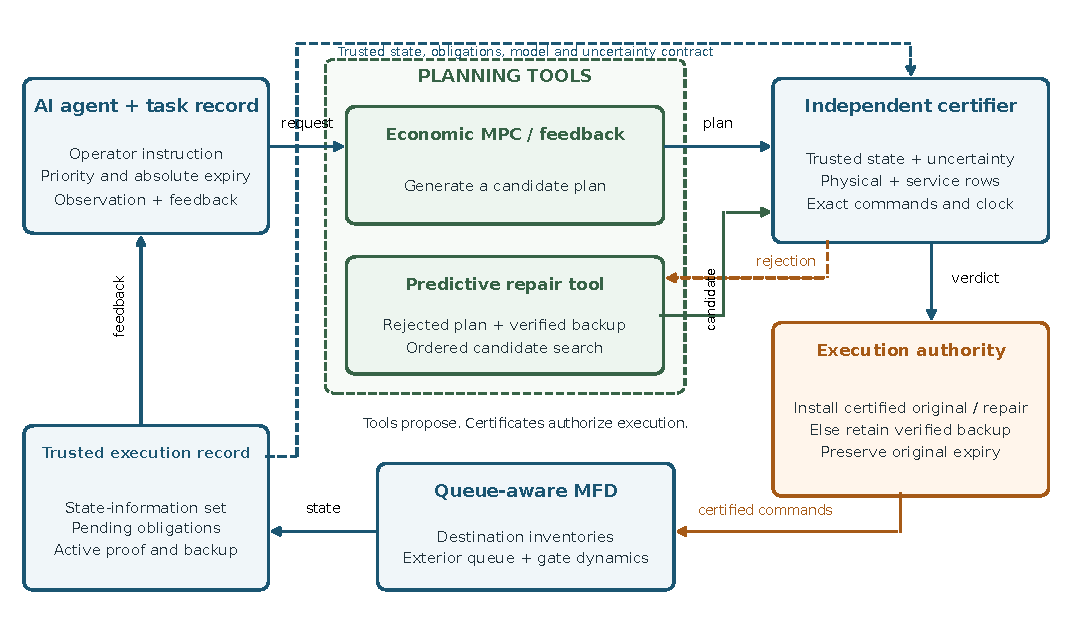
\includegraphics[width=0.98\textwidth]{figures/mfd_tool_architecture.pdf}
\caption{Agent interpretation, numerical planning and execution authority.
MPC, feedback rollout and predictive repair submit candidates to the same
certifier. Execution uses an accepted plan or the still-valid continuation.
The certified terminal policy supplies the expiry transition when available.
Memory and retrieved context affect requests, while the physical state,
obligations and uncertainty bounds determine whether a plan is accepted.}
\label{fig:new-architecture}
\end{figure}

\subsection{Executable plans and validity intervals}

A finite plan specifies command blocks $u=k_b+K_bx$ on absolute intervals.
Target-centered feedback has $k_b=u_b^\star-K_bx_b^\star$. Constant MPC
commands use $K_b=0$. An accepted replacement begins at its certified
installation time. Rejection preserves the unexecuted schedule, including
already authorized command changes, through its original expiry.
Proposal epochs, replacements and physical command changes are distinct:
a replacement can preserve its first command, and a rejected request changes
none. There are finitely many decision times in every bounded time interval. The terminal construction in
\appref{sec:terminal-backup} supplies conditions for continuation beyond expiry.

\section{Structure-Preserving Runtime Certification}
\label{sec:new-certification}

Authorizing a perimeter-control plan requires following the vehicles already
inside the regions together with those waiting for admission. Their
destination classes determine which regional inventories receive the waiting
vehicles. The certificate preserves this relationship while propagating
uncertainty and checking storage, command and service requirements over the
plan's full validity interval.

To construct the certification enclosure, we introduce the transformed state
\begin{equation}
\begin{aligned}
y=Lx=(&n_{11},n_{12},n_{10},n_{22}+(1-\pi)z,\\
      &n_{21}+\pi z,n_{20},z)^\top.
\end{aligned}
\label{eq:new-conservation-coordinates}
\end{equation}
The transformation combines each destination class that receives admitted
vehicles with the corresponding share of the exterior queue. As a result, the
admission flow cancels from the dynamics of these combined inventories and
remains explicitly only in the queue equation. This preserves the relevant
vehicle-conservation relationships during uncertainty propagation and reduces
conservatism in the certification analysis. The first six components of $y$
sum to the total system inventory $M=n_1+n_2+z$. The following construction
uses these coordinates to enclose each proposed plan and then carries the
resulting guarantees through sequential plan replacement and continued
execution after rejection.

\subsection{Plans, uncertainty, and transportation constraints}

A plan beginning at time $t_0$ consists of finitely many command blocks on
$[t_0,E]$, where $E$ is its absolute expiry. The residual bound $\bar w_x$ uses
the normalized flow units defined in Section~\ref{sec:benchmark-formulation}.
On block $b$, write
\begin{equation}
 u_b(x)=k_b+K_bx,
 \qquad \Lambda(t)=\widehat\Lambda(t)+w(t),
 \qquad |w(t)|\le\bar w_x.
 \label{eq:new-plan-data}
\end{equation}
In the primary two-region construction, the forecast $\widehat\Lambda$ is
continuous and piecewise affine, and $w$ is any measurable signal satisfying
the bound. Target feedback uses
$k_b=u_b^\star-K_bx_b^\star$. Constant MPC commands use $K_b=0$.
Furthermore, command changes preserve physical inventories.

The trusted physical limits are written as a finite set of affine
inequalities in the traffic state and gate commands. Each inequality is
called a constraint row:
\begin{equation}
 H_jx+J_ju\le \beta_j^{\rm phys},
 \qquad j=1,\ldots,n_c.
 \label{eq:new-physical-rows}
\end{equation}
These include nonnegative destination classes, regional and exterior storage,
gate boxes, and paired-gate differences. On block $b$ the row is
$h_{jb}^{\top}x\le\beta_{jb}$, with
$h_{jb}^{\top}=H_j+J_jK_b$ and $\beta_{jb}=\beta_j^{\rm phys}-J_jk_b$.
An operator service task consists of scheduled affine requirements
\begin{equation}
 g_r^{\top}x(T_r)\le\eta_r,
 \qquad r=1,\ldots,n_s.
 \label{eq:new-service-rows}
\end{equation}
Write $e_i$ for the $i$th standard coordinate vector. The Region~1 incident
deadline uses $g_r=100e_1$ and $\eta_r=2850$ vehicles
in the normalized state coordinates. A two-sided regional imbalance band is
represented by two rows. The operator fixes these rows, deadlines, and their
task version. They remain unchanged by the agent's memory or proposals.

\subsection{A computable enclosure that retains conservation structure}

Let $y=Lx$ be the invertible destination-class transformation in
\eqref{eq:new-conservation-coordinates}. If $b_a$ is the incidence vector of
admission in the physical balances, it satisfies
\begin{equation}
 Lb_a=-e_7,
 \qquad Le_7=(0,0,0,1-\pi,\pi,0,1)^\top.
 \label{eq:new-conservation-incidence}
\end{equation}
Admission cancels from the two combined inventories, leaving its nonsmooth
minimum explicitly only in the queue equation. Regional production retains
its dependence on the full transformed state.

For a fixed block, denote the physical field under its nominal forecast by
$f_b(x,t)$. The actual field is $f_b(x,t)+e_7w(t)$. Partition the plan at
command changes, forecast knots, service times, and prediction checkpoints.
On one interval $[t_l,t_l+h_l]$, choose a differentiable predictor $p_l(t)$
and inherited componentwise radii $r_l\ge0$ such that
$|L(x(t_l)-p_l(t_l))|\le r_l$. The implementation uses quadratic predictors.
For candidate outer radii $R_l>0$, the set
$p_l(t)+L^{-1}[-R_l,R_l]$ is a moving trial region around the predictor.
The radii are trial bounds on each component of the transformed prediction
error over this interval. Construct
the following bounds for every state and time in that region:
\begin{equation}
 \begin{aligned}
 a_{il}&\ge\sup (L D_xf_b L^{-1})_{ii},\\
 b_{ijl}&\ge\sup |(L D_xf_b L^{-1})_{ij}|\quad(j\ne i),\\
 \delta_{il}&\ge\sup_t |(L f_b(p_l(t),t)-L\dot p_l(t))_i|.
 \end{aligned}
 \label{eq:new-local-bounds}
\end{equation}
At an admission-branch boundary the Jacobian bounds include the convex hull
of both branch Jacobians. Verified exclusion of a branch throughout the
outer tube permits its removal from the bound. The diagonal bound $a_{il}$
retains its sign, while cross-component effects enter through magnitudes.

Define the nonnegative forcing and its scalar comparison solution by
\begin{align}
 c_{il}(R_l)&=\sum_{j\ne i}b_{ijl}R_{jl}
                 +\delta_{il}+|(Le_7)_i|\bar w_x,\nonumber\\
 \phi_{il}(s)&=e^{a_{il}s}r_{il}
                  +\chi(a_{il},s)c_{il}(R_l),\nonumber\\
 \chi(a,s)&=\begin{cases}(e^{as}-1)/a,&a\ne0,\\s,&a=0.\end{cases}
 \label{eq:new-component-comparison}
\end{align}
The interval passes its enclosure test when
\begin{equation}
 \max\{r_{il},\phi_{il}(h_l)\}<R_{il}
 \qquad\text{for every }i.
 \label{eq:new-self-inclusion}
\end{equation}
Continuous physical feasibility is verified by bounding the largest
value of each constraint expression over the trial region
\begin{equation}
 \sup_{t\in[t_l,t_l+h_l]}h_{jb}^{\top}p_l(t)
             +|h_{jb}^{\top}L^{-1}|R_l\le\beta_{jb}.
 \label{eq:new-affine-support}
\end{equation}
Absolute values of vectors and matrices are componentwise. If the next
predictor recenters by an amount bounded by $\delta^{\rm rec}_l\ge0$ in $L$ coordinates,
propagate $r_{i,l+1}=\phi_{il}(h_l)+\delta^{\rm rec}_{il}$. At a service checkpoint,
the resulting center $\widehat x(T_r)$ and radius $r(T_r)$ give the test
\begin{equation}
 g_r^{\top}\widehat x(T_r)+|g_r^{\top}L^{-1}|r(T_r)\le\eta_r.
 \label{eq:new-service-support}
\end{equation}

The following theorem connects these checks to physical and service feasibility for every trajectory allowed by the stated uncertainty bounds.

\begin{theorem}
\label{thm:new-plan-enclosure}
Consider the MFD field \eqref{eq:new-plant} with admission
\eqref{eq:new-admission}, a finite affine-command plan, and the uncertainty
class \eqref{eq:new-plan-data}. Let its initial information set be contained
in the initial predictor box. Suppose the bounds
\eqref{eq:new-local-bounds} hold for every state and time in each trial
region, and
\eqref{eq:new-self-inclusion} holds on every interval. Then the propagated
boxes contain every trajectory from that initial set under every allowed
residual. If \eqref{eq:new-affine-support} and
\eqref{eq:new-service-support} also pass, the trajectory satisfies every
physical row continuously through the plan's expiry and every included
service row at its deadline. At command or target changes, the inherited box
is propagated and the successor command rows are checked on that box.
\end{theorem}

\begin{proof}
On each predictor interval, let $z_e=L(x-p_l)$ be the transformed
prediction error and $v_i=|(z_e)_i|$ its componentwise magnitude.
Before any first contact with the
boundary of the trial region, the Jacobian and residual bounds give
\[
 \dot v_i\le a_{il}v_i+c_{il}(R_l)
 \quad\text{almost everywhere}.
\]
Multiplying by an exponential integrating factor and integrating gives
$v_i(t_l+s)\le\phi_{il}(s)$. The derivative
$\phi_{il}'(s)=e^{a_{il}s}(a_{il}r_{il}+c_{il}(R_l))$ does not change sign,
so its largest value occurs at an interval endpoint.
Condition \eqref{eq:new-self-inclusion} keeps both endpoint bounds
strictly below $R_{il}$. Continuity therefore rules out a first boundary
contact, and the trajectory stays inside the trial region.

At the next interval, the physical state is unchanged by a command or
target switch. The triangle inequality adds the predictor-center shift
to the propagated endpoint error, giving
\[
 r_{i,l+1}=\phi_{il}(h_l)+\delta^{\rm rec}_{il}.
\]
Repeating this argument over the finite partition proves containment
throughout the plan. Substituting $x=p_l+L^{-1}z_e$ into each constraint
then gives \eqref{eq:new-affine-support}; the endpoint box gives
\eqref{eq:new-service-support}. The constraints associated with a new
command are checked on the inherited state set at installation.
The complete derivation, including the admission-branch derivatives and
the comparison integral, is given in \appref{app:new-enclosure-proof}.
\end{proof}

The enclosure checks the plan using the forecast and its allowed arrival
residual, including any difference between that forecast and the arrival
level used to design a feedback controller. Target changes carry physical
uncertainty forward, while constant actuator rows are checked exactly. The
result supplies both continuous storage and gate checks and the regional
inventory bound at each service deadline.

\subsection{Positivity, queue comparison, and retained correlations}
\label{sec:structure-certificate}

The general enclosure developed above can be tightened by exploiting additional
structure of the traffic model. Each regional total equals the sum of its
destination-class inventories. Preserving these relationships supplies valid
information that can tighten the certification bounds.

Two useful properties follow directly from the traffic balances. First, if the
destination-class demands, offered arrivals, and constant commands are
nonnegative, then all six destination inventories and the exterior queue remain
nonnegative. For the polynomial completion factor used here,
$v(n)=G(n)/n$ is positive over the relevant domain, while conservation bounds
the total number of vehicles by the initial inventory together with cumulative
offered inflow. Thus, nonnegativity can be established independently of the
upper regional and queue-storage constraints.

Second, under a constant admission command, the queue dynamics are independent
of the regional states:
\begin{equation}
 \dot z=\widehat\Lambda(t)+w(t)-\min\{60z,120u_{02}\}.
 \label{eq:structure-scalar-queue}
\end{equation}
A scalar comparison argument therefore provides continuous lower and upper
bounds on $z$ from the extreme initial queue values and admissible arrival
bounds. Positivity directly verifies the lower bounds on the destination
classes and queue, while the scalar comparison checks the exterior-storage
constraint independently of the full state enclosure. Intersecting these
independently valid bounds with the propagated endpoint enclosure, and then
enclosing the intersection by an outward-rounded box, gives a first
refinement for the next propagation interval.

A second refinement propagates initial-state uncertainty through signed
generators, preserving dependencies among state components throughout the plan. On predictor interval $l$, write
\begin{equation}
 \begin{aligned}
 L(x-p_l)&=\Gamma_l(s)\xi+\zeta_l(s),\qquad |\xi|\le\mathbf1,\\
 \Gamma_l(s)&=e^{A_l^0s}\Gamma_l(0),\qquad |\zeta_l(0)|\le\rho_l.
 \end{aligned}
 \label{eq:structure-affine-set}
\end{equation}
Here, $\xi$ represents the common initial uncertainty, $\Gamma_l(s)$ propagates
its signed dependence through the interval, and $\zeta_l(s)$ collects the
remaining uncertainty not represented by those generators. The matrix
$A_l^0$ is held fixed over the interval to propagate the generator part, while
$\rho_l$ bounds the accumulated remainder.

Let $B_l(s)$ denote the mean-value Jacobian of the transformed dynamics over
the relevant state segment, and let
$\epsilon_l=L f_b(p_l,t)-L\dot p_l$ denote the predictor defect. The remainder
then satisfies the exact identity
\begin{equation}
 \begin{aligned}
 \dot\zeta_l={}&B_l(s)\zeta_l+(B_l(s)-A_l^0)\Gamma_l(s)\xi\\
              &+\epsilon_l+(Le_7)w.
 \end{aligned}
 \label{eq:structure-remainder-identity}
\end{equation}
A linear comparison system with nonnegative off-diagonal coefficients
(a Metzler matrix) bounds the magnitude of this remainder. The comparison
retains the signed diagonal contribution of $B_l$ and bounds cross-component
effects and forcing terms by their magnitudes. To bound the largest value of a constraint expression (its support), we
first combine the signed generator coefficients using that constraint's
coefficients, then apply absolute-value bounds to the resulting uncertainty
coefficients. This preserves cancellations between correlated state errors. Because
the same initial-uncertainty variables $\xi$ are retained across successive
intervals, correlations between regional totals and destination classes are
preserved, yielding tighter certification bounds.

\begin{proposition}
\label{prop:structure-plan}
Consider a finite plan of nonnegative constant commands with nonnegative
initial destination-class inventories and queue, nonnegative class demands and
offered arrivals, and a nonnegative completion factor for all nonnegative
regional accumulations. Suppose that, on each plan interval, the positivity
and scalar queue bounds, signed uncertainty propagation, remainder comparison,
and strict self-inclusion test in \appref{app:structure-proof} all hold. If the
corresponding physical and scheduled service checks pass, then every admissible
trajectory satisfies the physical constraints throughout the plan horizon and
all included service requirements at their scheduled deadlines. Across
interval boundaries, recentering and generator-rounding errors are absorbed
into the propagated remainder while the signed initial-state dependence is
retained.
\end{proposition}

\begin{proof}
When a destination-class inventory is zero, its outflow is zero and its
inflow is nonnegative under the stated sign assumptions. At an empty
queue, admission is zero and offered arrivals are nonnegative. The
detailed comparison in \appref{app:structure-proof} therefore establishes
nonnegative inventories independently of the upper storage limits.
The scalar queue equation also gives independent bounds by using the
smallest and largest initial queues with lower and upper arrival inputs.

For the remaining prediction error, the decomposition
$L(x-p)=\Gamma\xi+\zeta$ retains the same initial-uncertainty vector
$\xi$ throughout the plan. The generator $\Gamma$ propagates its signed
coefficients, while $\zeta$ collects the remaining error. The comparison
matrix has nonnegative off-diagonal entries, which allows a componentwise
bound
\[
 |\zeta(s)|\le e^{\overline M s}\rho+\Psi(s)b_\zeta.
\]
Together with the generator bound, this gives
$|L(x-p)|\le f+r^\zeta<R$, where $f$ bounds the generator contribution
and $r^\zeta$ bounds the remainder throughout the interval.
Continuity rules out a first contact with the
trial-region boundary. Substitution into each physical or service
constraint then bounds its largest possible left-hand side. Combining
the signed generator coefficients before taking absolute values preserves
their cancellations.

At each interval boundary, the remainder update includes both the
generator-rounding error and the change in predictor center, while the
same $\xi$ remains in use. Repeating these steps over the finite
partition proves the plan-wide guarantees. The complete inequalities
and their derivations are given in \appref{app:structure-proof}.
\end{proof}

The independent queue bound can tighten the region used to bound the
mean-value Jacobian. Its queue range must include every value between the
predictor queue and every queue state allowed by the true-state enclosure.
Both ends of this range must be retained. Generator and remainder bounds
are propagated separately, preserving their possible cancellation within the
total queue error. The two refinements supply complementary certificates
for the same physical contract. Their row supports determine the initial
uncertainty and nominal service margin that the operator can authorize.

\subsection{Certified execution of sequential agent proposals}
\label{sec:new-execution}

Sequential directives create a second transportation requirement: each new
plan inherits the vehicles and service deadlines left by the executed history.
A certificate for one proposed continuation becomes an execution guarantee
only when installation, replacement, and retention preserve that inheritance.

At installation, the supervisor records the certified plan together with the
state set from which it was verified, the authorized model and uncertainty
bounds, the applicable physical and service requirements, the exact command coefficients, the plan timing, the certified reachable sets
at subsequent checkpoints, and its expiry time. These quantities define the conditions under which the plan remains
authorized for execution.

\subsubsection{Admission and retained continuation}

At task activation, an initial verified plan is installed. At each subsequent
decision, the supervisor either installs a verified replacement beginning with
the proposed action or continues executing the remaining unexecuted portion of
the current verified plan.

If a proposed replacement is rejected, the currently verified plan continues
with its original command schedule, certified reachable set, modeling and
uncertainty assumptions, and absolute expiry time. The remaining plan may
include command changes that were already verified as part of that schedule.
New trusted measurements may further reduce the current uncertainty by
intersecting the certified reachable set with the set of states consistent
with those measurements.

In the signed-affine implementation, rejection continues the original
enclosure proof together with the history of control actions that have already
been executed. The remaining portion of the current verified plan is therefore
evaluated using the same correlated reachable set. The checkpoint box shown
at each decision time is used for reporting and inspection, while the retained
proof and execution history provide the basis for continuing the authorized
plan.

A replacement plan can start from a new trusted observation,
\[
\widehat x_i=x(t_i)+\nu_i,\qquad |\nu_i|\le d_i,
\]
and certifies the entire measurement-consistent set
\[
\mathcal I_i=\widehat x_i+[-d_i,d_i]
\]
at the actual installation time. This new observation-based set is verified
independently and may be larger than the reachable set associated with the
previous plan. The observation timestamp and error bound are treated as
trusted inputs to the certification process. When no new observation is
available, a propagated set containing every state allowed by the
incumbent's certificate and uncertainty bounds after its executed prefix
supplies the replacement information set, as in
Proposition~\ref{prop:planned-handover}.

For a certified plan $P$, let $\tau_P$ be its installation time and
let $\mathcal X_P$ be the trajectory family covered by its stored record:
\begin{equation}
\mathcal X_P=\{x_P(\cdot;x_0,w):
 x_0\in\mathcal I_{\tau_P},\ w\in\mathcal W_P\}.
\label{eq:execution-covered-family}
\end{equation}
Its expiry is $E_P$, and $\mathcal O_P$ contains its certified service
triples $(T_r,g_r,\eta_r)$. Theorems and propositions on one-plan
certification establish the physical rows and these service rows for every
member of $\mathcal X_P$. Retention restricts this same family to the
remaining interval, keeping its correlated history. A new hard requirement
is admitted only when the plan retained or installed covers it. A soft
priority request alone does not change the hard contract.

The following theorem carries these one-plan guarantees through successive
replacement or retention decisions.

\begin{theorem}
\label{thm:new-plan-closure}
Consider $t_0<\cdots<t_N<t_{N+1}=T$, including every plan-admission
decision and admission of a new service requirement on this finite
interval. Let $\mathcal X_0$ be the initial certified family, whose initial
set contains the actual state. For a proposal $\widehat P_i$, write
$\widehat{\mathcal X}_i=\mathcal X_{\widehat P_i}$. At $t_i$, accept it only when
$\mathsf{Cert}_{t_i}(\widehat P_i\mid\mathcal S_{t_i})=1$, its initial
set contains $x(t_i)$, and it covers all pending admitted requirements.
The selected trajectory family is
\begin{equation}
\mathcal X_i=\begin{cases}
\widehat{\mathcal X}_i,&\text{if the replacement is accepted},\\
\mathcal X_{i-1},&\text{otherwise},
\end{cases}\qquad i=1,\ldots,N.
\label{eq:execution-family-update}
\end{equation}
Let $P_i,E_i,\mathcal O_i$ be the plan, expiry and service rows stored
with this family. Assume the executed model, uncertainty and commands
satisfy its certificate, and
\[
t_{i+1}\le E_i,\qquad \mathcal O_{t_i}\subseteq\mathcal O_i,
\qquad i=0,\ldots,N,
\]
where $\mathcal O_{t_i}$ contains the pending admitted requirements.
Then
\begin{equation}
\begin{aligned}
H_jx(t)+J_ju^{\rm exec}(t)&\le\beta_j^{\rm phys},
 &&t\in[t_0,T],\\
g_r^\top x(T_r)&\le\eta_r,
 &&\text{admitted rows with }t_0\le T_r\le T.
\end{aligned}
\label{eq:execution-physical-service}
\end{equation}
Rows and uncertainty bounds refer to the applicable active certificate.
The finite guarantee extends to its expiry when no later plan is installed.
\end{theorem}

\begin{proof}
We show that each executed segment is covered by the certificate of the
plan selected for that segment. The initial certificate covers the actual
initial state and uncertainty, so it establishes the claim up to the first
decision.

At a decision time $t_i$, there are two cases. If the replacement is
rejected, the current plan keeps its original command schedule,
uncertainty assumptions, reachable-state history, and expiry. The actual
trajectory therefore continues as a member of the same certified family.
If the replacement is accepted, its initial set contains $x(t_i)$ and its
certificate covers every allowed future uncertainty realization. The
actual trajectory from $t_i$ onward is therefore covered by the new
family. In either case,
\[
 x|_{[t_i,t_{i+1}]}\in
 \{\widetilde x|_{[t_i,t_{i+1}]}:
          \widetilde x\in\mathcal X_i\}.
\]
This means that the executed segment agrees with a segment of a trajectory
covered by the selected certificate. The condition $t_{i+1}\le E_i$
ensures that this certificate remains valid until the next decision.

Repeating the argument at every decision proves the physical constraints
on all segments. At a switch, the physical state is continuous and the
constraints involving the new command are checked at installation, so the
constraints also hold at the switching time.

Every pending admitted service requirement is included in the selected
record by $\mathcal O_{t_i}\subseteq\mathcal O_i$. Thus each replacement
preserves its coverage, and each rejection preserves its existing proof.
At the deadline $T_r$, the covering certificate gives
$g_r^\top x(T_r)\le\eta_r$. This proves both parts of
\eqref{eq:execution-physical-service}.
\end{proof}


\subsubsection{Certification-aware predictive plan repair}
\label{sec:predictive-repair}

Retention preserves the obligation but may abandon a useful part of the
requested priority. We therefore add a certification-aware predictive filter, related
to the predictive safety-filter architecture of \cite{wabersich2021}, that
generates further proposals for the existing certifier. Its search variable
changes the entire finite command plan. Its certificate covers physical rows
and absolute service deadlines.

Consider the following decision record:
\[
\mathcal S_t=(\mathcal I_t,\mathcal W_t,\mathcal O_t,P_t^B,t,\mathsf v_t),
\]
where $\mathcal I_t$ is the current set of possible traffic states,
$\mathcal W_t$ is the uncertainty contract, $\mathcal O_t$ records the
outstanding service obligations, $P_t^B$ is the active verified plan,
and $\mathsf v_t$ identifies the installed model and constraint versions.
All repair candidates in this comparison use the same state information,
uncertainty bounds, obligations, backup plan, decision time, and model and
constraint versions. Let $E_B>t$ be the verified continuation's unchanged
expiry. Align the proposed and backup commands on a common
partition $t=\tau_0<\cdots<\tau_K=E_B$, subdividing constant blocks if
necessary. Write $P^0=(u_k^0)_{k=0}^{K-1}$ and
$P^B=(u_k^B)_{k=0}^{K-1}$. Every interpolated candidate preserves the
clock, block durations, state information, uncertainty bounds and service
requirements.
The repair family and finite grid are
\begin{equation}
\begin{aligned}
P(\lambda_{\rm rep})&=(1-\lambda_{\rm rep})P^0+\lambda_{\rm rep} P^B,\\
\mathcal G_{\rm rep}&=\{0=\lambda_{{\rm rep},0}<\cdots<\lambda_{{\rm rep},N_{\rm rep}}=1\}.
\end{aligned}
\label{eq:repair-family}
\end{equation}
The grid has $N_{\rm rep}+1$ weights, ordered from the proposal at zero
to the backup at one. Convex command constraints, including the box and directional
gate differences, are inherited from admissible endpoints. Nonlinear state,
queue and deadline constraints still require a new plan certificate.

Let $\mathsf{Cert}_t(P\mid\mathcal S_t)=1$ mean that the checker has certified
that the exact plan satisfies every physical constraint continuously and
every pending service requirement at its deadline over $[t,E_B]$, for all
initial states and uncertainty realizations specified by the decision record. A zero verdict leaves execution authority with the
verified continuation. Define
\begin{equation}
\lambda_{\rm rep}^*=\min\{\lambda_{\rm rep}\in\mathcal G_{\rm rep}:
                  \mathsf{Cert}_t(P(\lambda_{\rm rep})\mid\mathcal S_t)=1\}.
\label{eq:repair-selection}
\end{equation}
An ordered search tests every earlier grid point before selecting a later
one. The authority retains $P^B$ throughout this computation. The tool workflow
is: (i) certify the original proposal; (ii) on rejection, submit repair
candidates in increasing intervention order to the same checker; (iii)
install the first passing candidate only after validating its installation
binding; and (iv) retain the incumbent on exhaustion or timeout. A prior
verdict can be reused only for the identical plan and decision record. The endpoint
condition below uses a proof covering the \emph{same} snapshot. For an
enlarged observation box, the backup endpoint receives a fresh certificate
from that box, as in the numerical path audit.

The following theorem establishes finite search termination and the smallest change among certified candidates on the tested grid.

\begin{theorem}
\label{thm:repair-grid}
Suppose $\mathsf{Cert}_t(P^B\mid\mathcal S_t)=1$, $1\in\mathcal G_{\rm rep}$, and each
grid evaluation terminates. Ordered exhaustive search returns a certified
plan after at most $N_{\rm rep}+1$ evaluations. For any norm on the stacked command
vector, the first certified grid point minimizes
$\operatorname{dist}(P,P^0)=\|P-P^0\|$ over the certified points of this grid.
\end{theorem}
\begin{proof}
At the last grid weight, the interpolation equals the certified backup:
\[
 P(1)=P^B,
 \qquad \mathsf{Cert}_t(P^B\mid\mathcal S_t)=1.
\]
Hence at least one grid point passes. There are $N_{\rm rep}+1$ points,
and each evaluation terminates, so ordered search reaches a passing point
after at most $N_{\rm rep}+1$ evaluations. Because every earlier point has
already been tested, the returned weight $\lambda_{\rm rep}^*$ is the
smallest certified weight on the grid.

To relate this ordering to the command change, observe that
\[
 P(\lambda_{\rm rep})-P^0
 =\lambda_{\rm rep}(P^B-P^0).
\]
Multiplying a vector by a nonnegative scalar multiplies its norm by the
same scalar. Therefore,
\[
 \operatorname{dist}(P(\lambda_{\rm rep}),P^0)
 =\lambda_{\rm rep}\|P^B-P^0\|.
\]
This distance is nondecreasing in the grid weight, so the smallest
certified weight gives the smallest command change among certified grid
points. If $P^B=P^0$, every distance is zero and the conclusion still holds.
The proof uses the actual verdict at each tested point and allows passing
and failing verdicts in any order along the grid.
\end{proof}

The selected plan minimizes the change in command values among the tested
interpolations accepted by the checker. This minimum is defined by the
specified interpolation path, finite grid, and sufficient certification
test. Minimization over every interpolation weight requires additional
analysis of the certificate acceptance test. Section~\ref{sec:repair-results} uses ordered
exhaustive search. Earlier single-contract studies and their exhaustive-grid
search audits are preserved in the repository historical-study archive.

The following proposition shows that certified repair and retention on timeout preserve physical and service guarantees through the certified expiry.

\begin{proposition}
\label{prop:repair-execution}
Let $P^B$ be a valid incumbent on $[t,E_B]$, and consider an
installation time $t_a\in[t,E_B)$. A tested repair $P^R$ has expiry
$E_R>t_a$ and a completed-certificate time $t_{\rm ready}$, with
$t_{\rm ready}=\infty$ if no result is obtained. Assume the incumbent's
contract remains valid through preparation and installed records match the
actual time, model and coefficients. A repair installation requires
$x(t_a)\in\mathcal I_{t_a}$. All pending admitted service rows must be
covered by the selected record. Use
\begin{equation}
P^{\rm exec}=\begin{cases}
P^R,&t_{\rm ready}\le t_a\ \text{and}\quad
 \mathsf{Cert}_{t_a}(P^R\mid\mathcal S_{t_a})=1,\\
P^B,&\text{otherwise}.
\end{cases}
\label{eq:repair-installation-rule}
\end{equation}
The incumbent executes before $t_a$. Let $E_{\rm exec}$ be the selected
record's expiry. Then every physical row holds on $[t,E_{\rm exec}]$,
and every admitted service row in that record holds at its deadline.
Retention uses $E_{\rm exec}=E_B$ and the incumbent's original proof.
\end{proposition}

\begin{proof}
The currently accepted plan $P^B$ executes while the repair is prepared.
Its certificate therefore establishes the physical constraints and any
service requirements due before installation on $[t,t_a]$.

If the first case of \eqref{eq:repair-installation-rule} applies, the
repair certificate is ready by $t_a$, matches the actual installation
record, and covers the actual state because
$x(t_a)\in\mathcal I_{t_a}$. It therefore establishes the physical
constraints on $[t_a,E_R]$ and all remaining admitted service requirements
in its record. The state is continuous at installation, and the new
command constraints are checked there. Joining the certified intervals
$[t,t_a]$ and $[t_a,E_R]$ proves the claim with $E_{\rm exec}=E_R$.

Otherwise, $P^B$ continues with its original schedule and proof. Its
remaining trajectory is part of the family $\mathcal X_{P^B}$ already
covered by that proof, including the stored dependence on uncertainty.
Thus its physical and service guarantees remain valid through its
original expiry, giving $E_{\rm exec}=E_B$.

The condition $t_{\rm ready}\le t_a$ ensures that only a completed
certificate can authorize installation at $t_a$. An earlier computation
is usable at that time only when its certificate covers the actual
installation record, as required in the assumptions.
\end{proof}

Deployment also binds the certificate to the actual installation time and
installed command coefficients. A delayed installation receives a fresh
certificate from its activation state set, and implemented grid points are
ordered by their stored Euclidean command distances. \appref{app:repair-cost}
gives the complete timing and numerical-ordering conditions.

The next result gives conditions under which repair preserves certified operation beyond a finite plan's expiry.

\begin{corollary}
\label{cor:repair-recursive}
Use the terminal checker in \eqref{eq:terminal-checker} for repair
at the actual installation record. Suppose
$\mathsf{Cert}^{\mathcal K}_t(P^B\mid\mathcal S_t)=1$ and
$1\in\mathcal G_{\rm rep}$. Then the terminally certified grid set
\begin{equation}
\mathcal G_{\rm rep}^{\mathcal K}(t)=
\{\lambda_{\rm rep}\in\mathcal G_{\rm rep}:
\mathsf{Cert}^{\mathcal K}_t(P(\lambda_{\rm rep})\mid\mathcal S_t)=1\}
\label{eq:repair-terminal-grid}
\end{equation}
is nonempty. Under the initialization, uncertainty, installation and
local-finiteness assumptions of
Theorem~\ref{thm:backup-recursive-availability}, installing only members
of this set and retaining the incumbent on timeout preserves
\eqref{eq:terminal-global-guarantee}.
\end{corollary}

\begin{proof}
At weight one the interpolation equals the backup, $P(1)=P^B$.
The assumed terminal certificate for $P^B$ therefore gives
\[
 1\in\mathcal G_{\rm rep}^{\mathcal K}(t).
\]
Thus the terminally certified grid contains at least one candidate.

Every candidate selected from this grid has a certificate for its finite
physical constraints, all pending admitted service requirements, and its
transition to the terminal backup. In particular,
\[
 \mathcal R_{P(\lambda_{\rm rep})}(E_B)\subseteq\mathcal K.
\]
If each grid evaluation terminates, ordered search also selects the least
certified weight by Theorem~\ref{thm:repair-grid}. The continuation claim
holds for every selected member of the terminally certified grid.

If computation times out, the current plan keeps its original terminal
certificate, command schedule, and expiry. Therefore, successful repair
provides a new certified transition to the backup, while retention
preserves the existing transition. Under the stated initialization,
uncertainty, installation, and finite-installation assumptions, both cases
satisfy Theorem~\ref{thm:backup-recursive-availability}. That theorem gives
the physical and service guarantees in
\eqref{eq:terminal-global-guarantee}.
\end{proof}

Proposition~\ref{prop:repair-execution} covers the recorded finite-plan
interval. Corollary~\ref{cor:repair-recursive} adds certified continuation
beyond expiry through the terminal construction summarized next and proved in
\appref{sec:terminal-backup}. \appref{app:repair-cost} also gives
a finite-plan performance bound.

\paragraph{Future-dated certification during retained execution}
\label{sec:planned-handover}
At a preparation time $t$, the authority may choose a future activation
$t_a\in(t,E_B)$. Let $\mathcal R_B(t_a\mid\mathcal I_t)$ contain every state
reachable at that time by executing the incumbent's original absolute
schedule from $\mathcal I_t$ under any uncertainty realization allowed by
the active certificate. A
replacement can be verified in advance from an outer set
$\mathcal I_{t_a}^+\supseteq\mathcal R_B(t_a\mid\mathcal I_t)$, with commands
scheduled from $t_a$ and every remaining service time kept absolute.
Computation leaves the incumbent in force until this activation slot.

\begin{proposition}
\label{prop:planned-handover}
Suppose the incumbent has a valid certificate on $[t,E_B]$ and the
actual state at $t$ belongs to both $\mathcal I_t$ and its certified
reachable set. A replacement is certified from $\mathcal I_{t_a}^+$ on
$[t_a,E_R]$, where $E_R>t_a$, with
$\mathcal R_B(t_a\mid\mathcal I_t)\subseteq\mathcal I_{t_a}^+$.
Every service obligation pending at $t_a$ has its deadline in $[t_a,E_R]$
and is included in the replacement certificate. Assume that the model,
uncertainty, obligations and incumbent schedule used in propagation
remain valid through $t_a$, and that the executed model and uncertainty
satisfy the replacement contract through $E_R$.
If the replacement certificate is ready by
$t_a$ and the authority installs exactly its future-dated schedule at $t_a$,
physical constraints and admitted service rows hold through $E_R$.
If the certificate is unavailable or late and the incumbent contract
remains valid through $E_B$, retaining its original schedule preserves
its guarantees through $E_B$.
\end{proposition}
\begin{proof}
The current plan executes throughout preparation. Its certificate
therefore covers $[t,t_a]$, including every service requirement due in
that interval.

By definition, $\mathcal R_B(t_a\mid\mathcal I_t)$ contains every state
that can be reached at $t_a$ from the current information set under the
current plan and its allowed uncertainty. Since the actual state starts
in that set and the propagation assumptions remain valid,
\[
 x(t_a)\in\mathcal R_B(t_a\mid\mathcal I_t)
          \subseteq\mathcal I_{t_a}^+.
\]
Thus the replacement certificate covers the actual state at activation,
even though that state was unknown when computation began.

If the certificate is ready by $t_a$ and its specified schedule is
installed at exactly that time, its assumptions match the executed
replacement. It establishes the physical constraints and every remaining
admitted service requirement on $[t_a,E_R]$. Joining this interval to the
certified preparation interval gives the claim through $E_R$, including
the checked new-command constraints at activation.

If the certificate is unavailable or late, the current plan keeps its
original schedule, proof, and expiry. Under its continuing contract, the
executed trajectory remains covered through $E_B$. This is the retention
case of Theorem~\ref{thm:new-plan-closure}.
\end{proof}

The activation set can be a propagated outer box, optionally intersected
with a timestamped measurement set whose error bounds guarantee that it
contains the actual state. In the implementation, a checkpoint hull
is used as an input to a new proof. The retained incumbent continues
using its original correlated proof. Repair for the future slot aligns
the candidate and incumbent on their common absolute partition and
checks the endpoint independently from the future information set.
The finite-grid minimum then concerns the stored command vectors
evaluated for that slot. An authoritative task or model change during
preparation requires a new matching certificate before replacement.

\subsubsection{Continuation at plan expiry}
\label{sec:terminal-backup-main}

A finite-plan certificate covers execution through its expiry $E$, which
is preserved after rejection. Coverage beyond $E$ requires a replacement
installed by $E$ with a later certified expiry or a certified terminal
backup activated at $E$. If neither is available, the finite-plan result
establishes feasibility only through $E$.

The terminal-backup approach requires terminal certification of every
accepted plan. Its entire set of possible states at
expiry must lie in a robustly invariant set $\mathcal K$. From every state
in this set, the certified feedback policy $\mu_B$ keeps the state within this set and satisfies the physical
constraints for all future time under the stated uncertainty bounds. The finite-plan certificate must
also cover every service obligation pending at installation.
Rejection preserves the incumbent's certified terminal condition and
transition to this policy. An accepted replacement must establish its own
finite-horizon and terminal certification. Thus a certified continuation
is available at each decision time and at expiry, even if all later
proposals are rejected. \appref{sec:terminal-backup} states the invariant-set
condition and proves recursive availability.

We next extend the structure-preserving construction from the primary
two-region setting to networks with multiple exterior queues.




\subsection{Extension to networks with several entry queues}
\label{sec:network-extension}

With several entry queues, each admitted stream distributes waiting vehicles
among designated internal classes. Recording these receiving shares extends
the cancellation in \eqref{eq:new-conservation-incidence} to a network.
Let $c\in\R^q$ collect internal destination-class inventories,
$z\in\R^{n_q}$ the exterior queues, and $a\in\R^{n_q}$ their admitted flows. A fixed
allocation matrix $P_a\in\R^{q\times n_q}$ specifies which internal classes
receive each admission. For vehicle conservation, $P_a\ge0$ and
$\mathbf1_q^\top P_a=\mathbf1_{n_q}^\top$. Write the balances as
\begin{equation}
 \dot c=F(c,u,t)+P_a a,\qquad \dot z=\Lambda-a,
 \label{eq:network-class-queue}
\end{equation}
where $F$ includes internal demand, transfers and trip completion. The
regions may have different production functions and routing patterns.

The following proposition shows that the same queue--destination combination
used in the two-region model extends to multiple entry queues and confines the
explicit admission terms to the queue coordinates.

\begin{proposition}
\label{prop:network-localization}
For fixed $P_a$, the invertible coordinate map
\begin{equation}
 L_a=\begin{bmatrix}I&P_a\\0&I\end{bmatrix},\qquad
 y=L_a\begin{bmatrix}c\\z\end{bmatrix}
   =\begin{bmatrix}c+P_a z\\z\end{bmatrix}
 \label{eq:network-transform}
\end{equation}
gives
\begin{equation}
 \dot y_c=F(y_c-P_a z,u,t)+P_a\Lambda,\qquad
 \dot z=\Lambda-a.
 \label{eq:network-transformed-flow}
\end{equation}
Thus explicit admission terms occupy only the $n_q$ queue coordinates. No
invertible linear transformation can confine these $n_q$ independent channels
to fewer than $n_q$ scalar coordinates. Moreover,
$\mathbf1_q^\top y_c=\mathbf1_q^\top c+\mathbf1_{n_q}^\top z$, so the combined
inventories count all internal and waiting vehicles exactly once.
\end{proposition}

\begin{proof}
Because $P_a$ is fixed, differentiating $y_c=c+P_a z$ gives
\[
\begin{aligned}
 \dot y_c
 &=F(c,u,t)+P_a a+P_a(\Lambda-a)\\
 &=F(c,u,t)+P_a\Lambda.
\end{aligned}
\]
The admitted flow added to the regional classes cancels the same flow
removed from the queues. Substituting $c=y_c-P_a z$ gives
\eqref{eq:network-transformed-flow}. In matrix form, this cancellation is
\[
 L_a\begin{bmatrix}P_a\\-I\end{bmatrix}
 =\begin{bmatrix}0\\-I\end{bmatrix}.
\]
Thus the explicit admission terms appear only in the $n_q$ queue
coordinates.

To prove that fewer coordinates cannot suffice, consider the admission
matrix $\begin{bmatrix}P_a\\-I\end{bmatrix}$. Its columns are linearly
independent because its lower block is $-I$, so its rank is $n_q$.
Multiplication by an invertible coordinate map preserves this rank.
A matrix with nonzero entries in fewer than $n_q$ rows has rank smaller
than $n_q$. Consequently, an invertible transformation must retain at
least $n_q$ coordinates for these independent admission effects.

Finally, the allocation shares in each column of $P_a$ sum to one.
Therefore,
\[
\begin{aligned}
 \mathbf1_q^\top y_c
 &=\mathbf1_q^\top c+\mathbf1_q^\top P_a z\\
 &=\mathbf1_q^\top c+\mathbf1_{n_q}^\top z.
\end{aligned}
\]
Each waiting vehicle contributes a total share of one to the combined
inventories, so their sum counts every internal and waiting vehicle once.
\end{proof}

For independent queues with fixed block commands,
$a_i=\min\{k_i z_i,\kappa_i g_i\}$, where $g_i$ is the admission-gate command and
$k_i,\kappa_i\ge0$. Let $J_c=D_cF$, and let $D_a$ be a diagonal matrix of
admissible admission derivatives. The transformed Jacobian is
\begin{equation}
 J_y=\begin{bmatrix}J_c&-J_cP_a\\0&-D_a\end{bmatrix},
 \qquad (D_a)_{ii}\in[0,k_i].
 \label{eq:network-jacobian}
\end{equation}
The queue branches affect only diagonal entries. Cross-region coupling
remains in $J_c$ and $-J_cP_a$. Arrival residuals enter through $[P_a^\top,I]^\top w$.
These matrices supply the comparison, generator and output-support calculations
in the preceding construction in dimension $q+n_q$. The first-exit and
replacement arguments use the same inequalities. The network allocation
therefore specifies the coordinates needed to check regional service and
entry-storage rows on a common plan. The connected three-region test in
Section~\ref{sec:network-transfer-results} evaluates this extension on
identical physical plans in two coordinate systems.

The network construction also permits specified forecast jumps at partition
boundaries. Each comparison interval uses its own affine forecast segment.
Physical-state continuity supplies the inherited set at a jump. The
intervalwise comparison and support arguments therefore apply to the
piecewise-affine arrival profile in the transfer study.

Fixed allocation and independent admission are explicit modeling conditions.
Changing shares introduce additional terms, and receiving-supply coupling changes
the Jacobian blocks. \appref{app:network-transfer} states these corrections,
the transfer model and the dimension-dependent computation costs.



\section{Numerical Evaluation}
\label{sec:new-evidence}

The experiments address five questions. Does certification preserve a
useful controller's performance? What does transportation structure add to
the proof? How much priority can be recovered after a rejection? Can
successive tool requests preserve the inherited traffic contract? Can
execution continue during computation or under corrupted context? The comparisons below use the tasks
R, Q and D of Section~\ref{sec:benchmark-formulation}.

\subsection{Shared design and controller performance}
\label{sec:new-incident-protocol}
\label{sec:controller-benchmarks}

The queue-aware studies use the literature MFD, synthetic internal demands,
6000~veh/h base exterior arrivals and 2000-vehicle boundary storage of
\appref{app:new-model}. Arrival events increase the known mean by 20--50\%
for 30--60 minutes. Five-minute loading and recovery ramps are included in
the event duration. Each certificate encloses the specified initial-state
set and every measurable arrival residual within its bound. Matched replays
measure traffic cost on common initial states and residuals.

Task R compares the reproduced almost-smooth two-gate CLF of
\cite{zhong2018robust} with a local tracking MPC on the native four-state
plant. Twenty-four cases combine three initial regional-total pairs, two
destination splits, two gate intervals and constant or sinusoidal demand.
Both laws receive current demand, and MPC also receives the known future profile.
Task Q compares economic MPC following the predictive structure of
\cite{geroliminis2013mpc} with the specified queue/exit extension of that CLF.
Its twelve contracts combine four incident amplitudes with three durations,
one-vehicle all-state half-widths and a 300~veh/h residual bound.
The common minute-20 center is approximately
$(2102,2316,1421,1488,240,302,124)$ vehicles.

The decision clocks match their respective tasks. R replans every five
minutes with a 30-minute horizon over a 90-minute mission. Q and D test a
minute-20 replacement with five- and 35-minute command blocks ending at
minute 60. The eight-event compatibility study replans every five minutes
over two hours, with a one-hour prediction truncated at the endpoint.
Structure and binding-service tests use a one-hour mission. Detailed
controller settings, event definitions and independent checks are supplied
in \appref{app:reusable-benchmark}.

\begin{table}[t]
\centering\small
\caption{Controller performance and unchanged-plan certification. Controller
reductions use the stated CLF implementation as denominator. Q uses 960
matched feasible realizations. The compatibility grid uses nominal replay.}
\label{tab:benchmark-regulation-queue}
\label{tab:eight-event-compatibility-summary}
\begin{tabular}{@{}p{0.19\textwidth}p{0.29\textwidth}p{0.43\textwidth}@{}}
\toprule
Study & Controller result & Execution result\\
\midrule
R: 24 cases & Median $J_R$ reduction 73\% (range 21--96\%) & Both laws satisfy sampled physical limits in 24/24 cases.\\
Q: 12 contracts & Median TTS reduction 24\% (range 23--25\%) & 12/12 MPC plans certified and executed unchanged.\\
Compatibility: 8 events & Identical nominal/certified MPC trajectories & 192/192 admissions; 8/8 deadlines met; zero incremental realized TTS.\\
\bottomrule
\end{tabular}
\end{table}

Table~\ref{tab:benchmark-regulation-queue} separates the performance of the
implemented controllers from the effect of certification. Accepting an
admissible MPC plan preserves its commands and traffic benefit while adding
continuous uncertainty coverage and an explicit expiry.

\subsection{What conservation structure adds to certification}
\label{sec:structure-results}
\label{sec:new-mpc-results}
\label{sec:structure-online}
\label{sec:network-transfer-results}

These comparisons hold the physical plan, forecast and 15-second proof
partition fixed. For a held feedback plan and 2850-vehicle deadline, raw
accumulation coordinates leave the enclosure unresolved. Destination classes
give a Region-1 upper bound of 2220 vehicles. Adding waiting-inventory shares
reduces it to 2169, a 51-vehicle improvement. The complete coordinate
comparison is in Table~\ref{tab:new-coordinate-ablation}.

For the fixed two-block MPC plan, the regional/class half-width is $d$
vehicles and the queue half-width is $\min(d,10)$. $\bar w_{\rm veh}$ bounds the
exterior-arrival residual. Table~\ref{tab:structure-frontier} compares the
base interval enclosure, independent positivity/queue bounds and signed generators
of Proposition~\ref{prop:structure-plan}. Signed correlations extend the
largest tested certifiable regional width from 10 to 50 vehicles at a
60~veh/h residual. Positivity/queue bounds give tighter support for the
narrow box and larger residual, so the strengthened constructions are
complementary. A plan is accepted only if the certified bounds satisfy every physical
constraint and service requirement.

\begin{table}[t]
\centering\small
\caption{Certified Region-1 inventory bounds at minute 60 for a fixed
model predictive control (MPC) plan over minutes 0--60. Entries are rounded
upward in vehicles. The service limit is 2850. Here $d$ is the sensing
half-width of the first six state coordinates in \eqref{eq:new-plant}
(vehicles), the queue half-width is
$\min(d,10)$ vehicles, and $\bar w_{\rm veh}$ bounds the exterior-arrival
forecast residual in vehicles per hour (veh/h). Base interval uses the
componentwise enclosure in conservation coordinates. Positivity/queue adds
independently proved nonnegativity and scalar queue bounds. Signed also retains
shared initial-state dependence through signed generators and a bounded
remainder. A dash means the complete-plan certificate is unresolved.}
\label{tab:structure-frontier}
\setlength{\tabcolsep}{5pt}
\begin{tabular}{@{}rrrrr@{}}
\toprule
$d$ (veh) & $\bar w_{\rm veh}$ (veh/h) & Base interval & Positivity/queue & Signed\\
\midrule
1 & 60 & 1780 & 1729 & 1722\\
10 & 60 & 1845 & 1777 & 1725\\
50 & 60 & --- & --- & 1853\\
100 & 60 & --- & --- & ---\\
1 & 300 & --- & 2009 & 2256\\
25 & 300 & --- & --- & 2504\\
\bottomrule
\end{tabular}
\end{table}

For the 1700-vehicle service limit, tighter certified bounds reduce the
required planning margin under the same one-vehicle sensing half-widths
and 60~veh/h residual bound. On the same six-target menu, the base interval and
positivity/queue methods first certify a 1600-vehicle nominal target. Signed
generators also certify 1625, with a deadline bound below 1689 vehicles.
The clearance margin falls from 100 to 75 vehicles and nominal TTS by
0.90\% (41 veh-h). In repeated replacement, both certified initial targets
produce two admissions and ten rejections. The signed 1625-target plan
retains the 0.90\% TTS benefit and meets the hard deadline. The improvement
comes from the initial certified margin. \appref{app:structure-online-details}
reports the full target menu, adverse trajectory and eight-event comparison.

The same conservation construction transfers to fixed plans on connected
two- and three-region rings (six and twelve states). At the widest tested
regional-total half-width of 25 vehicles, the combined coordinates certify
the two-region plan with a 300~veh/h residual per queue and the
three-region plan with a 60~veh/h residual. Their largest regional
deadline bounds are 1552 and 2060 vehicles against a 2700-vehicle limit.
Ordinary class coordinates leave both proofs unresolved. Class half-widths
are $d/R$ and queue half-widths $\min(d,10)$ for $R$ regions. Successful
twelve-state proofs take 5.20--5.28 seconds for 120 intervals.
\appref{app:network-transfer} gives the complete sixteen-attempt sweep,
including the larger-residual cases, and the dimension-dependent cost.

\subsection{Deadline coverage and the price of priority recovery}
\label{sec:repair-results}

Task D holds the 30\% one-hour event and minute-20 center fixed. Its 72
development contracts vary the all-seven-state half-width
$d\in\{1,10,25,50\}$ vehicles, residual
$\bar w_{\rm veh}\in\{60,150,300\}$ veh/h, deadline
$\eta\in\{2750,2850,2950\}$ vehicles and Region-2 weight $p\in\{2,4\}$.
Eight held-out intermediate contracts use $d\in\{5,20\}$,
$\bar w_{\rm veh}\in\{100,225\}$, $\eta\in\{2800,2900\}$ and $p=3$.
Each constant plan has 640 replays: 128 initial-box corners and five
residual profiles. Full-scenario MPC constrains these scenarios plus the
nominal center forecast, with a one-vehicle planning margin. The independent
certificate covers the entire initial box and every bounded measurable
residual continuously through the minute-60 deadline.

\begin{table}[t]
\centering\small
\caption{Deadline-constrained Task D: 72 development and eight held-out
contracts over minutes 20--60. Entries count passing contracts out of 80.
Sample passes satisfy physical and service limits in all 640 replays
(128 initial-state corners times five arrival-residual profiles).
Family passes certify continuous physical limits and the minute-60 service
bound for every allowed initial state and residual. MPC means model predictive control.
Nominal MPC plans from the state-set center with zero residual.
Five-scenario MPC adds the all-low/all-high states with both constant
residual extremes. Full-scenario MPC uses all 640 combinations plus the
center forecast. All minimize center-forecast priority cost. Checked-repair
entries count all certified outputs: unchanged proposals and checked
interpolations toward a backup. Reserve refresh constructs a new certified
backup for nominal-plan repair when the old continuation fails its check.}
\label{tab:benchmark-deadlines}
\begin{tabular}{@{}lrr@{}}
\toprule
Planning/execution option & Sample passes & Family passes\\
\midrule
Nominal MPC & 36/80 & 36/80\\
Five-scenario MPC & 40/80 & 40/80\\
Full-scenario MPC & 80/80 & 44/80\\
Nominal MPC with checked repair & 74/80 & 74/80\\
Full-scenario MPC with checked repair & 74/80 & 74/80\\
Repair with checked reserve refresh & 80/80 & 80/80\\
\bottomrule
\end{tabular}
\end{table}

Table~\ref{tab:benchmark-deadlines} distinguishes sampled feasibility from
family certification. Fresh checking certifies the existing continuation in 68 of the 80
contracts. Ordered repair produces a certified plan in 74. Newly constructed
reserves pass certification in all twelve contracts where the original
continuation fails its check, enabling repair in the remaining six. This tests
the same-contract certified-endpoint premise of
Theorem~\ref{thm:repair-grid}. The physical CBF-QP separately passes physical
rows in 80/80 matched adverse runs and service in 44/80. Its denominator is
one adverse trajectory per contract. Its instantaneous barriers protect
storage and gates, while service remains a scheduled evaluation row.

The common conflict $(d,\bar w_{\rm veh},\eta,p)=(1,300,2850,4)$, at the all-high
corner and constant positive residual, makes these distinctions concrete
(Table~\ref{tab:benchmark-conflict}). Nominal MPC violates storage and the
deadline. The physical CBF protects storage but misses the deadline.
Retention and checked repair satisfy both. Full-scenario MPC passes this
trajectory but its sufficient family proof remains unresolved. Checked
repair supplies that stronger execution certificate.

\begin{table}[t]
\centering\footnotesize
\caption{Matched adverse realization, minutes 20--60. TTS is total
time spent in the regions and exterior queue. $J_D$ weights Region~2 by
$p=4$. Both use veh-h. Costs and counts are rounded to whole
units. Peak queue is the maximum exterior count $100z$. $100n_1(E)$ is the
Region-1 count at deadline $E=60$ minutes. Their limits are 2000 and 2850
vehicles. P/S lists physical/service outcomes: P=pass, F=fail. Cert.
reports full-family certification: Yes=certified, No=unresolved,
dash=not assessed by that checker.
MPC means model predictive control, and CBF means control barrier function.
Retained continuation follows the previous certified plan. Nominal-plan
and Full-scenario repair interpolate their MPC proposals toward it.}
\label{tab:benchmark-conflict}
\setlength{\tabcolsep}{3pt}
\begin{tabular}{@{}lrrrrcc@{}}
\toprule
Policy & TTS & $J_D$ & Peak queue & $100n_1(E)$ & P/S & Cert.\\
\midrule
Nominal MPC & 3300 & 6328 & 2180 & 2852 & F/F & No\\
Physical CBF & 3295 & 6376 & 1844 & 2917 & P/F & ---\\
Retained continuation & 2695 & 6814 & 194 & 1727 & P/P & Yes\\
Nominal-plan repair & 3097 & 6427 & 1683 & 2310 & P/P & Yes\\
Full-scenario MPC & 3267 & 6357 & 1999 & 2848 & P/P & No\\
Full-scenario repair & 3075 & 6453 & 1547 & 2314 & P/P & Yes\\
\bottomrule
\end{tabular}
\end{table}

For the nominal, retained and repaired plans $P^0,P^B,P^R$ on a common
realization $\omega$, report percentage reduction in priority cost $\Delta J_\omega$, percentage change in queue-inclusive delay $\Delta D_\omega$ and
recovered requested benefit $B_\omega$:
\begin{equation}
\begin{aligned}
\Delta J_\omega&=100\frac{J_D(P^B;\omega)-J_D(P^R;\omega)}{J_D(P^B;\omega)},\\
\Delta D_\omega&=100\frac{J_Q(P^R;\omega)-J_Q(P^B;\omega)}{J_Q(P^B;\omega)},\\
B_\omega&=\frac{J_D(P^B;\omega)-J_D(P^R;\omega)}{J_D(P^B;\omega)-J_D(P^0;\omega)}.
\end{aligned}
\label{eq:benchmark-repair-metrics}
\end{equation}
Positive $\Delta J_\omega$ means a reduction in priority cost relative
to retention. Positive $\Delta D_\omega$ means an increase in
queue-inclusive delay. Both changes are percentages. The recovered
benefit is reported as $100B_\omega$ percent.
Across 24,320 paired realizations from the 38 original-continuation repair
contracts, every requested-benefit denominator is positive. Median priority
improvement is 5.7\%, delay increase 16.1\%, and recovered benefit 91.7\%.
Thus retention minimizes TTS in the displayed conflict, while repair serves
more of the requested Region-2 preference. Compared with the nominal
certified MPC tool, the stronger scenario tool's priority improvement ranges
from $-0.41$\% to $+4.30$\%, with median zero. Selecting the lowest center-forecast
cost among certified tools before replay yields 61 nominal-MPC plans,
13 full-scenario plans and 6 refreshed reserves. \appref{app:reusable-benchmark}
gives the paired evaluation protocol. Complete per-realization costs and
earlier single-contract results are preserved in the repository.

\subsection{Successive planning-tool changes}
\label{sec:sequential-handover-results}

Task D also tests successive planning requests within one incident. A
certified weight-$p=4$ ordinary-MPC repair is active at minute 20. At
minute 25 the agent requests the remaining constant command from the
previously computed $p=2$ full-scenario MPC. At minute 30 it requests the
remaining command from the $p=4$ nominal MPC. The hard physical limits and
absolute minute-60 Region-1 deadline stay fixed. The requested Region-2
weight follows $4\to2\to4$ across the three execution intervals. Each
activation information set is obtained by propagating the active plan's
reachable set under the existing information contract and enclosing it
by an outward physical box.
Archived planner outputs define this deterministic request sequence, isolating
physical admission from language interpretation.
Replacement is checked from that box through minute 60. A failed request
leaves the current plan's original correlated proof, command schedule and
expiry in force.

\begin{table}[t]
\centering\small
\caption{Successive changes in deadline-constrained Task D. Case entries
are stored contract identifiers. The 25/30 column gives the decisions at
minutes 25 and 30: A=accept the replacement, R=retain the current plan.
Unchecked feasible and Certified feasible count replays satisfying both
physical limits and the minute-60 service requirement out of 640 matched
initial-state/arrival realizations. TTS means total time spent, including
the exterior queue, over minutes 20--60, in veh-h.
Median TTS F/U/C gives three medians in order: F=retain the fixed initial
certified plan, including its scheduled command changes; U=execute both
requested replacements without checking; C=execute only certified
replacements and retain the current plan after rejection. Medians use all
640 replays, including infeasible unchecked runs. D015, D027 and D071 were
preselected. D025 is the first storage-violation case found in the complete
matched-pair scan.}
\label{tab:sequential-handover}
\setlength{\tabcolsep}{4pt}
\begin{tabular}{@{}lcccc@{}}
\toprule
Case & 25/30 & Unchecked feasible & Certified feasible & Median TTS F/U/C\\
\midrule
D015 & A/A & 640/640 & 640/640 & 3196/3081/3081\\
D027 & A/R & 640/640 & 640/640 & 3037/3081/2717\\
D071 & R/R & 640/640 & 640/640 & 3169/3094/3169\\
D025 & A/R & 512/640 & 640/640 & 2963/3070/2719\\
\bottomrule
\end{tabular}
\end{table}

The three preselected pairs in Table~\ref{tab:sequential-handover} share
their hard contracts within each weight-$4$/weight-$2$ pair. D015 admits
both changes and executes exactly the requested schedule. D027 admits the
first change and retains it after the second request fails the sufficient
service enclosure, although the sampled unchecked path remains feasible.
D071 retains the initial plan at both requests when the propagated outer
boxes include inadmissible physical states.

The complete development grid contains 36 matched weight pairs. 30 have
the archived certified source plans required for this sequence. Unchecked
switching overfills exterior storage in three of these 30 cases. All three
were passed through the full sequential checker. In the first case by
numeric ID, D025, the minute-25 scenario-MPC command is certified from
the inherited state set. The minute-30 nominal command fails the queue
storage check. Unchecked execution reaches 2005.59 vehicles against the
2000-vehicle queue limit on a constant-high residual realization,
confirmed by independent adaptive integration. Retaining the accepted
scenario-MPC suffix gives 640/640 physically and service-feasible replays,
with median queue-inclusive TTS 8.2\% below holding the initial certified
plan. Its changing-priority cost is 5.2\% above unchecked switching,
recording the cost of declining the later soft-priority request. The other
two overflow cases, D043 and D061, and all request outcomes appear in
\appref{app:sequential-handover}. These studies assume that plans take effect at the specified times.
The following subsection accounts for computation while the accepted
plan continues.

\subsection{Execution during computation and corrupted context}
\label{sec:delayed-handover-results}
\label{sec:task-state-live}
\label{sec:queue-live-pilot}
\label{sec:primary-memory-pressure}

\subsubsection{Execution during computation}

Future-dated handover exercises Proposition~\ref{prop:planned-handover}.
Seventeen contracts (eight development extremes, the displayed conflict and
eight held-out cases) use one-, two- and five-minute preparation slots.
The incumbent executes while its information set is propagated under the
existing observation and uncertainty contract. A replacement is optimized and certified from the entire
future box through the unchanged minute-60 deadline. Late or unsuccessful
preparation leaves the original correlated proof, schedule and expiry active.

Table~\ref{tab:delayed-handover} records 30 timely replacements and 21
retentions across 51 preparation cases, with all 32,640 trajectories
feasible. Three one-minute results are late. Longer slots provide more
computation time but also widen the propagated box and shorten the remaining
service horizon. Conversion to a physical box discards class correlations, which can
prevent certification of a replacement.
The incumbent remains covered by its original certificate in those cases.

\subsubsection{Interpretation under corrupted context}

The agent studies use \texttt{gpt-5.4-mini-2026-03-17}, reasoning disabled,
and strict tool schemas. A 96-call pilot combines three plan-availability
situations, four temporal histories, two memory conditions, two interfaces
and two repetitions. Histories include interruptions, nested restoration and
exact expiry. Poisoned tool memory attempts to change priorities or bypass
admission. Pilot choices route precomputed plans. Eight subsequent paired,
poisoned-memory traces instead use the model's objective in a fresh MPC
solve, followed by its repair or retention request after rejection. Thirteen
live calls complete these traces. Each authorized plan has 640 replays.

\begin{table}[t]
\centering\small
\caption{Delayed activation and agent decisions. Top: Handover slot is
preparation time after minute 20. Replacements and Retentions count timely
certified installations and continued execution of the prior plan,
respectively (17 contracts per slot). Each row has
$17\times640=10{,}880$ replays through minute 60.
Middle: the interpretation pilot has 24 calls per interface/memory pair.
History only supplies observations and interaction memory. Task record
also supplies the active priority and its expiry. Clean memory is
unaltered. Poisoned memory contains misleading instructions. Objective
correct means agreement with the active priority. Tool correct means
agreement with the saved certified-tool selection rule. Bottom: each
interface has four traces and $4\times640=2560$ replays. Objective correct
assesses initial requests. Repairs executed counts traces installing a
certified grid repair. Feasible trajectories satisfy physical and service
constraints.}
\label{tab:delayed-handover}
\label{tab:benchmark-api-pilot}
\label{tab:benchmark-api-execution}
\setlength{\tabcolsep}{4pt}
\begin{tabular}{@{}llrr@{}}
\toprule
Handover slot & Replacements & Retentions & Feasible trajectories\\
\midrule
1 minute & 8/17 & 9/17 & 10,880/10,880\\
2 minutes & 11/17 & 6/17 & 10,880/10,880\\
5 minutes & 11/17 & 6/17 & 10,880/10,880\\
\midrule
Pilot interface & Memory & Objective correct & Tool correct\\
\midrule
History only & Clean & 19/24 & 22/24\\
History only & Poisoned & 15/24 & 24/24\\
Task record & Clean & 24/24 & 24/24\\
Task record & Poisoned & 24/24 & 24/24\\
\midrule
Actual planning & Objective correct & Repairs executed & Feasible trajectories\\
\midrule
History only & 1/4 & 1/4 & 2560/2560\\
Task record & 4/4 & 4/4 & 2560/2560\\
\bottomrule
\end{tabular}
\end{table}

Providing the authoritative task record improves identification of the
active operator objective in these small paired examples. Numerical certification enforces the unchanged physical and service
requirements on every authorized plan. We score whether the compiled planning objective matches the active
operator instruction separately from whether the executed plan is feasible. Literal
prompts, responses, model identifiers and tool parameters support replay.
\appref{sec:supp-execution} gives the current agent experiment protocol.
Earlier API and local-model protocols are preserved in the repository
historical-study archive with their original model versions, clocks and
denominators.

\section{Operational Insights and Implementation}
\label{sec:new-discussion}

\subsection{The operator's decision}

The benchmark separates controller selection from permission to execute its
next plan. Regional regulation tests recovery to an accumulation target.
Queue-inclusive planning accounts for waiting outside the network. Deadline
replacement tests whether a new preference can inherit an existing service
obligation. Acceptance records the sensing and forecast bounds and the plan's expiry,
while leaving its commands unchanged. In the matched comparisons, MPC plans accepted without repair produce
the same traffic performance as the original proposed schedules.
Sequential tool changes add a second test: the candidate must be verified
from the traffic state inherited from the executed prefix. In the matched
incident, this check admits an earlier scenario-MPC command and keeps its
verified suffix when a later nominal request fails the boundary-storage check.

When a request conflicts with inherited limits, retained execution and
checked repair answer different operational preferences. Retention preserves
the authorized schedule. Repair serves more of the requested regional
priority at a measured queue-inclusive delay cost. Such priorities can
represent regional clearance commitments, incident-response access or an
operator directive to protect a receiving district. The hard service deadline
remains binding during these soft-objective changes. A physical barrier and
a deadline-aware plan certificate consequently answer different questions.

Conservation-aware proof representations change the uncertainty sets and
initial service margins for which the same plan can be certified. A widened
information contract may require a freshly checked reserve before repair.
Computation then takes place under the active schedule, with the proposed
activation time and propagated state set included in the replacement proof.
The task record separately preserves priorities and their absolute expiries.
Together these elements make priority revision an explicit, checkable
transportation decision.

\subsection{Information requirements and model scope}
\label{sec:information-model-scope}

The experiments use a literature MFD and synthetic demands constructed from
a nominal operating record. Planners receive the event mean. Certificates
treat production, destination fractions, internal demand, release rate and
gate capacity as fixed parameters. They enclose the specified sensing and
exterior-arrival uncertainty. The reported traffic costs apply to these model assumptions, available
information and controller settings. The native CLF reproduction, queue/exit
extension, local MPC and physical CBF are specified implementations with
their objective, information and constraint coverage stated explicitly.

Destination-class observability is a substantive deployment requirement.
The initial one-vehicle box and wider tested boxes are assumed information
contracts. Regional totals can correspond to several destination mixtures.
An estimator must therefore deliver a joint set containing the actual class inventories
and queue, accounting for bias, calibration and observation timestamps.
The queue-capped structure sweep and all-state deadline sweep use distinct
sets. MFD, routing and release uncertainty affect the vector field and its
derivatives through additional channels that require validated bounds on
every proof interval. Allocation corrections are given in
\appref{app:network-assumptions}.

Trajectory replay checks the selected initial states and arrival profiles.
The continuous certificate covers the full specified uncertainty set. Their gap in the full-scenario experiment identifies where tighter
nonlinear dependency propagation or planning margins could enlarge admission.
Recorded violations distinguish a physically unsuccessful plan from one
whose sufficient certificate remains unresolved. The live-model study is a
small, version-specific demonstration of interpretation and tool execution.
Released requests and responses permit decision replay. Hardware and load
likewise condition the reported preparation times. The connected-network
study tests transfer and proof cost under its own routing and uncertainty
contracts.

The numerical experiments evaluate finite plans through their recorded
expiries. Indefinite continuation through the terminal backup additionally
requires the invariant backup, terminal landing and obligation coverage of
\appref{sec:terminal-backup}. Sustained arrivals must be compatible with
finite storage and achievable discharge.

\subsection{Operational setup and reuse}

An implementation needs production and destination-flow models, storage and
receiving-supply limits, information sets assumed to contain the actual state and
forecast-error sets assumed to contain the arrival residuals, absolute
service deadlines and a verified initial continuation. Changed authoritative
tasks or model versions require matching certificates. Scheduling must budget
propagation, planning, checking and actuation while the incumbent remains in
force. If a result arrives too late, the active plan continues with its original
commands, proof and expiry.

The three task definitions and released fixtures let later methods compare
regulation error, TTS, priority cost, storage and service satisfaction,
certificate availability and computation on shared problems. The experimental
appendices provide the protocols needed to assess the reported results. The
repository provides commands, raw calls, proof records, per-realization outputs
and earlier comparisons.

\section{Conclusions}
\label{sec:new-conclusion}

This paper develops a framework for checking agent-proposed urban
perimeter-control plans before execution. It verifies physical constraints
and service deadlines within the stated traffic model and uncertainty
bounds, using vehicle conservation and the links between boundary queues and
regional traffic to tighten bounds on future states. Plans that pass
certification can be executed unchanged, and checked repair searches for
certified alternatives. Rejected or late replacements leave the previously
accepted plan in use through its certified validity interval. When the
required terminal conditions are also certified, feasible operation can
continue beyond plan expiry. Numerical studies show reduced conservatism and
recovery of feasible plans through repair. Further experiments examine
successive plan changes, connected networks, computation delays, and errors
in the information given to the agent, with certified execution maintained
in the tested cases.

Future work will focus on estimating vehicle counts by region and
destination from traffic measurements and calibrating the associated
uncertainty bounds. Another direction is to establish uncertainty bounds
that capture differences between the traffic model and observed network
behavior. We will also study when new plans should take effect, accounting
for sensing, computation, and actuation time, traffic uncertainty, and
remaining service deadlines. These developments will support evaluation of
the framework in operational traffic networks.

\FloatBarrier
\section*{CRediT authorship contribution statement}
\textbf{Ali Eslami:} Conceptualization, Methodology, Software, Validation,
Formal analysis, Investigation, Data curation, Visualization,
Writing and editing.
\textbf{Jiangbo Yu:} Supervision, Review and editing.

\section*{Declaration of competing interests}
The authors declare that they have no known competing financial interests or
personal relationships that could have appeared to influence the work
reported in this paper.

\section*{Data and code availability}
Reproducibility materials include the traffic models, planning and
certification implementations, experiment protocols, stored agent requests
and responses, proof records, and trajectory-replay outputs described in the
experimental appendices. The materials are maintained at
\url{https://github.com/AlienEslami/agentic-perimeter-runtime-certification}.


\appendix
% Use appendix letters for equations while retaining full appendix section titles.
\renewcommand{\theequation}{\Alph{section}.\arabic{equation}}
\section{Initial-Plan Data and Certificate Construction}
\label{app:new-model}

\subsection{Queue-aware model and reference controllers}

The seven-state model in \eqref{eq:new-plant} uses vehicle counts normalized
by 100 vehicles and time measured in hours. In the primitive-demand order
$(11,12,10,22,21,20)$, the fixed internal demands are
\begin{equation}
\begin{aligned}
\boldsymbol d^{\rm int}=(&74.85630,37.42815,18.714075,\\
              &44.85630,7.42815,0.748563).
\end{aligned}
\label{eq:new-incident-demands}
\end{equation}
The displayed decimals are rounded. The exact stored binary coefficients
define the implemented field and are included in every proof. With base
exterior admission 60 and $u^\star=(0.5,0.5,0.5,0.52)$, the regional
state $(30,30,15,15,5,5)$ is an equilibrium and the exterior queue is 2.
The total base offered input is 244.031538 normalized units/hour, of which
the exterior stream supplies 24.587\%. These demands are reconstructed from
the specified equilibrium and then remain fixed across all events and
reference choices. The separate stationary record is retained in the earlier-study research package.

To construct a feedback reference with regional totals $(N_1,N_2)$ and
reference exterior arrival $A$, let $v_i=v(N_i)$, set
$u_{20}^\star=0.52$, $z^\star=2$ and $\pi=1/2$. Steady class balances give
\begin{equation}
\begin{aligned}
q_{11}^\star&=d^{\rm int}_{11}+d^{\rm int}_{21}+\pi A,&
q_{22}^\star&=d^{\rm int}_{22}+d^{\rm int}_{12}+(1-\pi)A,\\
n_{11}^\star&=q_{11}^\star/v_1,&
n_{22}^\star&=q_{22}^\star/v_2,\\
u_{12}^\star&=\frac{d^{\rm int}_{12}+d^{\rm int}_{10}}{G(N_1)-q_{11}^\star},&
n_{10}^\star&=\frac{d^{\rm int}_{10}}{u_{12}^\star v_1},\\
n_{20}^\star&=\frac{d^{\rm int}_{10}+d^{\rm int}_{20}}{0.52v_2},&
n_{21}^\star&=N_2-n_{22}^\star-n_{20}^\star,\\
u_{21}^\star&=\frac{d^{\rm int}_{21}+\pi A}{v_2n_{21}^\star},&
u_{02}^\star&=A/120.
\end{aligned}
\label{eq:new-targets}
\end{equation}
Linearization uses the strict capacity branch at the reference. The
continuous-time LQR weights are
$Q=\operatorname{diag}(1,1,0.1,0.1,0.1,0.1,2)$ and $R=3000I_4$.
The installed negative feedback gains give
$u=u^\star+K(x-x^\star)$ for reference triples
$(N_1,N_2,A)=(20,22,72),(22,24,78),(24,26,84)$.
Certification uses the actual event forecast, accounts for its difference
from the controller-design arrival $A$, and includes the full equilibrium
residual computed with the stored coefficients.

The controller-design search also includes $(18,20)$, reference arrivals
$60,72,78,84$, and input penalties $3000,30000,300000,3000000$.
All 64 outcomes are retained. The three controllers are the lowest-cost candidates for three
distinct target pairs on the selection grid. Two additional 45-minute
events broaden the validation set.

\section{Enclosure Proof and Verified Implementation}
\label{app:new-enclosure-proof}

\subsection{Conservation coordinates and nonsmooth flow}

The model equations and destination definitions are specified in
Section~\ref{sec:new-problem}. \appref{app:new-model} supplies the controller-design
parameters. For admission fraction $\pi$, its physical incidence is
$b_a=(0,1,0,1-\pi,0,0,-1)^\top$. The transformation
\eqref{eq:new-conservation-coordinates} has inverse
\begin{equation}
 \begin{aligned}
 n_1&=y_1+y_2+y_3,&
 n_2&=y_4+y_5+y_6-y_7,\\
 n_{11}&=y_1,&n_{22}&=y_4-(1-\pi)y_7,\\
 n_{10}&=y_3,&n_{20}&=y_6,\qquad z=y_7.
 \end{aligned}
 \label{eq:new-inverse-coordinates}
\end{equation}
Direct multiplication gives \eqref{eq:new-conservation-incidence}. Adding
each receiving-class equation to its share of $\dot z=\Lambda-a$ cancels
admission, while $n_1+n_2+z=\sum_{i=1}^{6}y_i$. These identities use a fixed
destination fraction and explicit conservation of waiting vehicles.

The class production $q_{ij}=n_{ij}G(n_i)/n_i$ is evaluated through the
polynomial speed $G(n_i)/n_i$, extended continuously at zero. Under affine
feedback the two admission branches are affine in the physical state, and
their minimum is continuous and locally Lipschitz. Consequently the
closed-loop field is locally Lipschitz in state and measurable in time.
Bounded measurable residuals give unique absolutely continuous solutions
locally. The compact enclosures below continue them throughout each verified
finite plan.

At a branch surface, the generalized Jacobian is contained in the convex hull
of the smooth branch Jacobians. This follows from the definition as limits
of classical Jacobians at differentiability points and their convex hull.
Both branches must be bounded on any outer predictor set intersecting that
surface. Outward bounds that establish a strict branch gap can instead
restrict evaluation to the feasible branch. The inequalities
\eqref{eq:new-local-bounds} remain valid for every convex combination of the
retained Jacobians.

\subsection{Componentwise first-exit argument}

Consider one interval $[t_l,t_l+h]$, and omit its index from the
bounds. We first show that the true state stays inside the trial
region around the predictor. Define the transformed prediction error
by
\[
 z_e(t)=L\bigl(x(t)-p(t)\bigr).
\]
Initially, $|z_e(t_l)|\le r<R$. Suppose that some component of
$|z_e|$ reaches its trial bound $R_i$ for the first time during
the interval. Before this first boundary contact, the segment
joining $p(t)$ to $x(t)$ lies entirely inside the trial region.

The difference between the true and predicted dynamics satisfies
\begin{equation}
 \dot z_e=A(t)z_e+\epsilon(t)+(Le_7)w(t),
 \label{eq:new-error-dynamics}
\end{equation}
where
\[
 \epsilon(t)=Lf_b(p(t),t)-L\dot p(t),
 \qquad |\epsilon_i(t)|\le\delta_i.
\]
Equation \eqref{eq:new-error-dynamics} holds almost everywhere:
any exceptional times form a set of measure zero and do not affect
the integration below.

The matrix $A(t)$ represents the change in the nominal dynamics
between the predictor and the true state. More precisely, it lies
in the convex hull of the transformed generalized Jacobians along
the segment. These matrices account for the derivatives of all
relevant admission branches, including points where the active
branch changes. Taking their convex hull allows weighted averages
with nonnegative weights summing to one. Since every included
matrix satisfies \eqref{eq:new-local-bounds}, these averages satisfy
\[
 A_{ii}(t)\le a_i,
 \qquad |A_{ij}(t)|\le b_{ij}\quad(j\ne i).
\]

For $v_i(t)=|(z_e(t))_i|$, the other components satisfy
$v_j(t)\le R_j$ before boundary contact. Consequently,
\begin{equation}
 \dot v_i\le a_i v_i+c_i(R)
 \quad\text{almost everywhere before boundary contact}.
 \label{eq:new-error-comparison-proof}
\end{equation}
Here $c_i(R)$ bounds the combined effect of the other error
components, the predictor residual, and the arrival uncertainty.
The inequality also holds almost everywhere when $v_i=0$.

Multiplying by $e^{-a_i(t-t_l)}$ and integrating yields
\[
\begin{aligned}
 v_i(t_l+s)
 &\le e^{a_i s}v_i(t_l)
      +\int_0^s e^{a_i(s-\tau)}c_i(R)\,d\tau\\
 &\le e^{a_i s}r_i+\chi(a_i,s)c_i(R)
  =\phi_i(s).
\end{aligned}
\]
Since
\[
 \phi_i'(s)=e^{a_i s}\bigl(a_i r_i+c_i(R)\bigr),
\]
its derivative does not change sign. Thus its largest value on
$[0,h]$ occurs at an endpoint. Condition
\eqref{eq:new-self-inclusion} gives
\[
 \phi_i(s)\le\max\{r_i,\phi_i(h)\}<R_i.
\]
By continuity, this bound also holds at any proposed first
boundary contact, contradicting $v_i=R_i$. Therefore, the
trajectory remains inside the trial region throughout the interval.
The bounded enclosure and the stated regularity assumptions also
ensure that the solution exists through the interval endpoint.

At $t_{l+1}=t_l+h$, the error relative to the current predictor is
bounded by $\phi(h)$. The physical state remains continuous across
a command change. If the next predictor uses a different center,
the predictor-center shift is bounded by
\begin{equation}
 \delta^{\rm rec}_l\ge
 |L(p_l(t_{l+1})-p_{l+1}(t_{l+1}))|.
 \label{eq:new-recentering-bound}
\end{equation}
The triangle inequality therefore gives
\[
\begin{aligned}
 |L(x(t_{l+1})-p_{l+1}(t_{l+1}))|
 &\le \phi(h)+\delta_l^{\rm rec}\\
 &=r_{l+1}.
\end{aligned}
\]
This supplies the initial error bound for the next interval.
Repeating the argument over the finite partition proves
containment throughout the plan.

It remains to verify the constraints. For a physical constraint
$h_{jb}^{\top}x\le\beta_{jb}$, write $x=p+L^{-1}z_e$. At each time,
\[
 h_{jb}^{\top}x
 \le h_{jb}^{\top}p(t)+|h_{jb}^{\top}L^{-1}|R.
\]
Condition \eqref{eq:new-affine-support} bounds the right-hand side
by $\beta_{jb}$ throughout the interval. At a service deadline,
the propagated endpoint box similarly gives
\[
 g_r^{\top}x(T_r)
 \le g_r^{\top}\widehat x(T_r)
      +|g_r^{\top}L^{-1}|r(T_r)
 \le\eta_r,
\]
where the final inequality is
\eqref{eq:new-service-support}. At command changes, the inherited
box is also checked against the constraints associated with the
new command. Hence all physical constraints hold continuously,
and every included service requirement holds at its deadline.

If a verified implementation
uses distinct invertible transforms before and after a boundary, the valid
transfer is
\begin{equation}
 r_{\rm next}\ge
 |L_{\rm next}L_{\rm old}^{-1}|\phi(h)
 +|L_{\rm next}(p_{\rm old}-p_{\rm next})|.
 \label{eq:new-coordinate-transfer}
\end{equation}
All centers in this expression are evaluated at the same boundary time.
An initial physical box centered at $p(t_0)$ with radius $d_x$ is enclosed
in the transformed coordinates by $r_0\ge|L|d_x$.

\subsection{Verified numerical bounds and exact constant commands}

The implemented piecewise quartic field and quadratic predictor produce a
defect polynomial of degree at most eight on each affine-forecast interval.
The verifier collects coefficients in the conservation coordinates before
interval evaluation. Outward arithmetic bounds the polynomial ranges,
Jacobian entries, inverses where needed, and scalar comparison functions.
Propagation intervals are split at the exact times of forecast knots,
command-block boundaries, and service deadlines. Predictors and trial radii
may be generated numerically. Plan acceptance requires the outward-rounded
trajectory bounds and constraint checks to pass.

For $a\ne0$, the comparison integral can be evaluated as
\begin{equation}
 \chi(a,h)=\frac{\operatorname{expm1}(ah)}{a},
 \qquad \chi(0,h)=h.
 \label{eq:new-stable-comparison}
\end{equation}
This is the same integral as \eqref{eq:new-component-comparison}.
The \texttt{expm1} evaluation avoids cancellation when the bound on a
queue-Jacobian diagonal entry is close to zero, including when its exact
value is zero. Regression checks compare positive, negative, zero,
near-zero, and subnormal rates with high-precision evaluation.

For $K_b=0$, actuator rows are constants. The installed binary command
coefficients are interpreted as exact binary rationals, and the gate
residuals are evaluated exactly:
\begin{equation}
 \begin{gathered}
 u_i,\quad 1-u_i\quad(i=1,\ldots,4),\\
 \tfrac34\pm(u_{21}-u_{12}),\qquad
 \tfrac34\pm(u_{20}-u_{02}).
 \end{gathered}
 \label{eq:new-exact-actuator-residuals}
\end{equation}
A nonnegative exact residual satisfies its original closed inequality.
An outward lower floating-point representation preserves this conclusion,
including exact zero. The verifier applies this rule only after checking
that the gain is identically zero. The twelve state, class, regional, and
storage support calculations remain unchanged. Regression checks
include exact boundary commands and one-unit-in-the-last-place violations
of box and paired-gate rows. The proof identifier includes both the command
coefficients and this exact support rule.

\subsection{Proof records, retained portions, and task coverage}

A plan record binds its initial set, physical coefficients and constraints,
command blocks, forecast and residual, absolute times, service rows,
propagated checkpoint sets, and expiry. Each checkpoint identifies its
parent proof. After a rejected replacement, the state set and commands are the corresponding
remaining portion of that same record. Restricting a universally
verified trajectory family to its remaining interval preserves containment
and every pending service check. This is the invariant used by
Theorem~\ref{thm:new-plan-closure}.

For clarity, a replacement accepted before a task's last deadline must
include every pending service time, even when it uses a different nominal
forecast or prediction horizon. Its actual disturbance must belong to that
replacement's specified family. Until replacement, the current proof's own
assumptions must remain valid. A forecast update, sensing error outside the
certified bound, or a changed receiving-supply model is part of a new
certification record. The execution theorem is applied with a valid record
at each activation. An installation set containing the actual state can be obtained by
propagating the active plan's bounds during computation and intersecting
that enclosure with a measurement set that also contains the actual state. Without an accepted replacement, the finite-horizon guarantee remains
valid through the active plan's original certified expiry.

\section{Structure-Preserving Reachable Sets}
\label{app:structure-proof}

\subsection{Independent positivity and queue information}

Recall $v(n)=G(n)/n$, extended polynomially at zero. The stored and derived
class balances in \eqref{eq:new-plant} give
\begin{equation}
 \begin{aligned}
 \dot n_{12}&=d^{\rm int}_{12}-u_{12}v(n_1)n_{12},\\
 \dot n_{21}&=d^{\rm int}_{21}+\pi a-u_{21}v(n_2)n_{21}.
 \end{aligned}
 \label{eq:structure-derived-classes}
\end{equation}
Together with the four stored-class equations and queue equation, these
balances show that a zero destination-class inventory has nonnegative
inflow and zero outflow whenever the other inventories, commands, primitive
demands, and offered arrivals are nonnegative and $v\ge0$. At $z=0$,
admission is zero and offered arrivals are nonnegative. For the installed
binary coefficients $(\alpha_2,\alpha_1,\alpha_0)=(0.0014877,-0.29815,15.0912)$, exact arithmetic gives
$\alpha_2>0$ and $4\alpha_2\alpha_0-\alpha_1^2>0$. Completing the square proves
\begin{equation}
 v(n)=\alpha_2\left(n+\frac{\alpha_1}{2\alpha_2}\right)^2+
                    \frac{4\alpha_2\alpha_0-\alpha_1^2}{4\alpha_2}>0.
 \label{eq:structure-positive-factor}
\end{equation}
The minimum is approximately $0.15314$ h$^{-1}$. This algebraic continuation
establishes positivity independently of the requested jam and storage bounds.
To make this argument precise, let $N_-(t)$ be the
sum of the magnitudes of all negative class inventories and the negative
queue part. Local Lipschitz continuity gives, locally,
\[
 \dot N_-(t)\le L_-N_-(t)
 \quad\text{almost everywhere}
\]
for a finite constant $L_-$. Since $N_-(t_0)=0$, integration gives
$N_-(t)\le e^{L_-(t-t_0)}N_-(t_0)=0$. All classes and the queue therefore
remain nonnegative. Conservation also gives
\[
 0\le M(t)\le M(t_0)+
 \int_{t_0}^t
 \bigl(d^{\rm int}_1+d^{\rm int}_2+\Lambda(s)\bigr)\,ds.
\]
Bounded arrivals keep this total finite on each finite interval, so the
solution can be continued throughout the plan. These arguments establish
the lower inventory limits independently of the upper storage limits.
The nine lower state and class constraints follow from these independent
nonnegativity bounds.

For constant gates, the scalar queue equation preserves the order of
solutions when their initial queues and arrival inputs are ordered. The
smallest initial queue with the lower arrival input bounds every allowed
trajectory from below; the largest initial queue with the upper input
bounds it from above. With constant extremal arrival $\lambda$ and
$\kappa=120u_{02}$, its branch solutions are
\begin{equation}
 \begin{aligned}
 z(s)&=\lambda/60+(z_0-\lambda/60)e^{-60s}
                    &&(60z\le \kappa),\\
 z(s)&=z_0+(\lambda-\kappa)s &&(60z\ge \kappa).
 \end{aligned}
 \label{eq:structure-queue-flows}
\end{equation}
Interval exponential/logarithmic evaluation encloses branch crossings.
Affine forecast intervals use their outward extremal arrivals when the common
branch remains unresolved. Exact forecast and command cutpoints are retained.
This supplies endpoint and continuous bounds for all measurable allowed
residuals. The queue-storage requirement is tested against their upper bound.
If this continuous enclosure proves a common branch and the forecast is
$\ell_0+\ell_1s$, sharper endpoint comparisons use
\begin{equation}
\begin{aligned}
 z(h)&=e^{-60h}z_0+(\ell_0\pm\bar w_x)\varphi_1+\ell_1\varphi_2
       &&\text{(supply)},\\
 z(h)&=z_0+(\ell_0\pm\bar w_x-\kappa)h+\ell_1h^2/2
       &&\text{(gate)},\\
 \varphi_1&=(1-e^{-60h})/60,\qquad
 \varphi_2=(h-\varphi_1)/60.
\end{aligned}
\end{equation}
The minus and plus signs give the lower and upper solutions. Only the
endpoint interval is intersected with these bounds. The independently
established continuous enclosure remains in force.

An initial physical box must itself satisfy class/queue nonnegativity. This
is checked by exact supports of the class map. Subsequent verified boxes may
be intersected with independently established positivity and queue intervals,
then enclosed outward. This operation preserves the reachable family and
includes recentering error. The Jacobian bounds within a step must cover the entire segment between
the predictor and the true state. For the queue coordinate, use the convex
hull of the predictor queue range and the independently bounded continuous
true queue range, intersected with the original trial enclosure. This
restricted enclosure contains every required predictor-to-state segment
and is used below to bound the Jacobians. Admission branches
can be excluded when this enclosure rules them out, including when the
predictor lies outside the true queue range.

\subsection{Signed propagation and robust variational remainder}

Consider one interval, omit $l$, and let $\mathcal J_\varpi$ bound each retained
transformed branch Jacobian on that region. In
\eqref{eq:structure-affine-set}, the same vector $\xi$ represents the
initial uncertainty throughout the plan. The generator $\Gamma$ propagates
its signed coefficients, while $\zeta$ collects the remaining error.
The remainder may depend on $\xi$. Choose any fixed matrix $A^0$ and
differentiate the decomposition to obtain
\eqref{eq:structure-remainder-identity} exactly. For a fresh physical box
$x(t_0)\in\widehat x+[-d_x,d_x]$, initialize $p(t_0)=\widehat x$,
$\Gamma(0)=L\operatorname{diag}(d_x)$ and $\rho=0$ before numerical
conversion. Generator conversion error is absorbed outward into $\rho$.
Precisely, the mean-value matrix satisfies
$L[f_b(x,t)-f_b(p,t)]=B(s)L(x-p)$, with $B(s)$ in the convex hull of
the retained transformed branch Jacobians along the predictor-to-state
segment. These Jacobian bounds cover the complete transformed error
$L(x-p)=\Gamma\xi+\zeta$, including both its generator and remainder
contributions.
Define a comparison matrix $\overline{M}$ with nonnegative off-diagonal
entries, called a Metzler matrix, and a nonnegative forcing bound
$b_\zeta$ by
\begin{equation}
 \begin{aligned}
 \overline{M}_{ii}&=\max_\varpi\sup(\mathcal J_\varpi)_{ii},\\
 \overline{M}_{ij}&=\max_\varpi\sup|(\mathcal J_\varpi)_{ij}|\quad(i\ne j),\\
 (b_\zeta)_i&\ge\max_\varpi\sup_{J\in\mathcal J_\varpi,\,F\in\mathcal F}
                  \sum_j|[(J-A^0)F]_{ij}|\\
             &\hspace{1em}+\delta_i+|(Le_7)_i|\bar w_x,
 \end{aligned}
 \label{eq:structure-metzler}
\end{equation}
where $\mathcal F$ contains $e^{A^0s}\Gamma(0)$ for all $s\in[0,h]$,
and $\delta_i\ge\sup_s|\epsilon_i(s)|$. Weighted averages of the
retained branch Jacobians satisfy the same bounds. Applying them to the
remainder identity gives
\[
 \frac{d}{ds}|\zeta|\le\overline M|\zeta|+b_\zeta
 \quad\text{almost everywhere}.
\]
Since $\overline M$ has nonnegative off-diagonal entries,
$e^{\overline M s}$ has nonnegative entries. Componentwise comparison and
integration therefore give
\[
 |\zeta(s)|\le e^{\overline M s}\rho+
             \int_0^s e^{\overline M(s-\tau)}b_\zeta\,d\tau.
\]
Thus
\begin{equation}
 |\zeta(s)|\le e^{\overline{M}s}\rho+\Psi(s)b_\zeta,
 \qquad \Psi(s)=\int_0^s e^{\overline{M}v}\,dv.
 \label{eq:structure-remainder-bound}
\end{equation}
The integral $\Psi(s)$ is componentwise increasing. Individual entries
of the exponential may decrease, so the contribution from the inherited
remainder must be bounded over the full interval. With outward bounds
\begin{equation}
 \begin{aligned}
 f_i&\ge\sup_{s\in[0,h]}\sum_j|(e^{A^0s}\Gamma(0))_{ij}|,\\
 r_i^\zeta&\ge\sup_{s\in[0,h]}(e^{\overline{M}s}\rho)_i
                            +(\Psi(h)b_\zeta)_i,
 \end{aligned}
 \label{eq:structure-continuous-radii}
\end{equation}
the test $f+r^\zeta<R$ keeps every error component strictly inside the
trial enclosure. If a component first reached the boundary, continuity
would give the same strict interior bound there, a contradiction. The
positivity and
scalar queue bounds used here are established independently of this
containment test.

For a constraint $a_x^\top x\le b_x$, substitution of
$x=p+L^{-1}(\Gamma\xi+\zeta)$ gives
\[
 a_x^\top x\le a_x^\top p+
 \|a_x^\top L^{-1}\Gamma\|_1+
 |a_x^\top L^{-1}|\,|\zeta|.
\]
Here $|\xi|\le\mathbf1$ bounds the generator contribution by the sum of the
absolute values of its combined coefficients. Combining the signed
coefficients first preserves their cancellations. Taking the stated time
bounds gives the following upper bound on the constraint's left-hand
side throughout the interval:
\begin{equation}
 \sup_s a_x^\top p(s)+
 \sup_s\|a_x^\top L^{-1}e^{A^0s}\Gamma(0)\|_1+
 |a_x^\top L^{-1}|r^\zeta.
 \label{eq:structure-signed-output}
\end{equation}
At a scheduled service deadline, the endpoint generator and remainder
give the corresponding bound. Independently established positivity,
queue, and exact constant-command bounds may also verify their
corresponding constraints. Each constraint can use its tighter valid bound.

Let $\widehat\Gamma$ be the stored binary generator at the next endpoint,
and let $d_\Gamma$ enclose the row sums of
$|e^{A^0h}\Gamma(0)-\widehat\Gamma|$. Since $|\xi|\le\mathbf1$,
\[
 |(e^{A^0h}\Gamma(0)-\widehat\Gamma)\xi|\le d_\Gamma.
\]
Adding this generator-rounding error to the endpoint remainder and the
predictor-center shift in \eqref{eq:new-recentering-bound} gives
\begin{equation}
 \rho^+\ge d_\Gamma+e^{\overline{M}h}\rho+\Psi(h)b_\zeta+\delta^{\rm rec}.
 \label{eq:structure-endpoint-update}
\end{equation}
It retains the same $\xi$ and includes all numerical conversion errors.
The scalar queue bound constrains the total physical queue error. Its
generator and remainder summands can cancel, so neither is separately
contracted by that total-error bound. The propagated set therefore
provides a valid starting set for the next interval. Repeating the
argument over the finite partition proves
Proposition~\ref{prop:structure-plan}.

\subsection{Validated matrix functions and execution records}

For any matrix $A$, $\alpha\ge\|A\|_\infty$, $\sigma=\alpha h$ and series order
$p$, the exponential and integral tails obey
\begin{equation}
 \begin{aligned}
 \left\|e^{Ah}-\sum_{k=0}^p\frac{A^kh^k}{k!}\right\|_\infty
       &\le e^\sigma\frac{\sigma^{p+1}}{(p+1)!},\\
 \left\|\int_0^h e^{As}\,ds-
          \sum_{k=0}^p\frac{A^kh^{k+1}}{(k+1)!}\right\|_\infty
       &\le he^\sigma\frac{\sigma^{p+1}}{(p+2)!}.
 \end{aligned}
 \label{eq:structure-matrix-tails}
\end{equation}
The second inequality follows by integrating the first pointwise tail and
using $e^{\alpha s}\le e^{\alpha h}$. The implementation uses $p=18$.
Signed coefficients $a_x^\top L^{-1}(A^0)^k\Gamma(0)$ are formed before
interval time evaluation. For the transformed constraint row $a_x^\top L^{-1}$ and generator column $\Gamma_j$,
the transformed tail is bounded by
$\|a_x^\top L^{-1}\|_1\,e^\sigma \sigma^{p+1}/(p+1)!\,\|\Gamma_j\|_\infty$.
Outward rounding covers every retained coefficient, tail, product and sum.

On rejection, the accepted plan continues with its original generator and
remainder history, structural bounds, command schedule and expiry. Its
endpoint box $|L(x-p)|\le |\Gamma|\mathbf1+\rho$ contains the reachable
states but omits correlations represented by that history. Continuing the
existing proof uses the stored history. A fresh proof can use the correlated
set or a containing box, provided it verifies the full chosen set. A
timestamped observation box supplies an independent set containing the
actual state under its measurement assumptions. The replacement certificate
covers that entire set and every pending deadline. These continuation and
replacement cases establish the induction in
Theorem~\ref{thm:new-plan-closure} for the structure-preserving implementation.

\section{Network Allocation Conditions}
\label{app:network-assumptions}

\subsection{Allocation changes and branch structure}

Proposition~\ref{prop:network-localization} uses constant allocation shares.
For a known differentiable $P_a(t)$, differentiating $y_c=c+P_a(t)z$ gives
\begin{equation}
 \dot y_c=F(c,u,t)+P_a(t)\Lambda+\dot P_a(t)z.
 \label{eq:network-varying-allocation}
\end{equation}
With fixed reference coordinates $y_c=c+P_0z$ and actual shares $P_a(t)$,
the corresponding expression is
\begin{equation}
 \dot y_c=F(c,u,t)+P_0\Lambda+(P_a(t)-P_0)a.
 \label{eq:network-uncertain-allocation}
\end{equation}
The extra terms enter the predictor and uncertainty enclosure. At a specified
piecewise-constant share change, physical inventories remain continuous but
coordinates change. Propagate the same initial uncertainty symbol through
$\Gamma^+=L_a^+(L_a^-)^{-1}\Gamma^-$, and bound the remainder by
$|L_a^+(L_a^-)^{-1}|\rho^-$ plus outward conversion and predictor-recentering
error. The implemented
transfer study uses constant shares and retains one coordinate map throughout.

For fixed commands and independent queues, bounding each queue's diagonal
Jacobian entry separately gives valid comparison bounds for
\eqref{eq:network-jacobian}, independently of simultaneous admission-branch
combinations. The predictor-defect calculation enumerates combinations of
branches that the local tests have not excluded, with at most $2^{n_q}$
combinations. Shared receiving capacities, regional-state-dependent
admission, and feedback gates require Jacobian bounds that include their
actual couplings.

\section{Task-State Transitions and Temporal Consistency}
\label{app:task-state-compiler}

\subsection{State, operations and temporal consistency}

The canonical record $\theta_i$ contains an active regional priority and a
last-in, first-out stack of suspended priorities, each with region, label and
absolute expiry. Network operation is the default. Before a proposal at $t_i$,
$\mathsf{Age}_{t_i}$ removes an expired active task and pops expired predecessors until
an unexpired task is restored or the stack is empty. Aging compares absolute expiries with the current time. Enumerate the
active task and then the suspended tasks from most recent to oldest, with
expiries $\tau_1^{\mathrm{exp}},\ldots,\tau_m^{\mathrm{exp}}$. The first
surviving entry is
\begin{equation}
k_t=\min\{k\in\{1,\ldots,m\}:\tau_k^{\mathrm{exp}}>t\}.
\label{eq:task-age-survivor}
\end{equation}
If this set is empty, aging returns network operation. Otherwise entry
$k_t$ becomes active, its older predecessors remain suspended, and all
original expiries are preserved. On the active task and suspension stack,
\begin{equation}
\mathsf{Age}_t(\mathsf{Age}_s\theta)=\mathsf{Age}_t\theta,
\qquad t\ge s.
\label{eq:task-age-composition}
\end{equation}
Indeed, entries removed at $s$ have expiry at most $s\le t$ and cannot
become the first surviving entry at $t$. Setting $s=t$ proves idempotence,
so aging both between proposals and before compilation is consistent.
Audit-history timestamps are separate from this task-state identity.

For a parsed operation
$r_i^A$,
\begin{equation}
 \theta_i^+=\mathsf{UpdateTask}(\mathsf{Age}_{t_i}\theta_i,r_i^A),\qquad
 (j_i,\Delta_i)=\mathsf{SelectTask}(\theta_i^+,t_i),
 \label{eq:task-state-compiler}
\end{equation}
Here $\mathsf{UpdateTask}$ updates the parsed task record and
$\mathsf{SelectTask}$ selects its objective and remaining duration.
The compiler $\mathsf{Comp}$ also forms the numerical planning request.
The index $j_i$ selects the soft objective. A regional task expiring at $\tau_i^{\mathrm{exp}}$
has $\Delta_i=\tau_i^{\mathrm{exp}}-t_i>0$. Network operation has $\Delta_i=0$.
The same expiry rule applies between proposals.

\begin{table}[t]
\centering\small
\caption{Compiler transitions. Only the listed fields accompany the operation
name. Durations/extensions are integer minutes in $[1,120]$. Nonempty labels
contain at most 80 characters.}
\label{tab:task-state-operations}
\begin{tabular}{@{}p{0.14\textwidth}p{0.22\textwidth}p{0.56\textwidth}@{}}
\toprule
Operation & Additional fields & Transition at time $t$\\
\midrule
Set & Region, duration, label & Clear the stack and install a task expiring at
$t+D/60$, for duration $D$ minutes.\\
Interrupt & Region, duration, label & Save the active task with its original
expiry and install a temporary task expiring at $t+D/60$, for duration $D$ minutes.\\
Continue & None & Preserve the surviving task and expiry.\\
Extend & Minutes & Add $D/60$ hours to the active task's expiry, for extension $D$ minutes.\\
Resume & None & Restore the latest unexpired saved task. If none survives,
clear the interruption. With no stack or interruption, keep the current task.\\
Cancel; network & None & Clear active and suspended tasks and use network operation.\\
\bottomrule
\end{tabular}
\end{table}

The compiler rejects extra fields, extension of an absent task and
interruption depth above four. Invalid operations create no new planning
request. The canonical record derives from schema-valid model operations,
independently of evaluation labels and physical-plan admission. A valid operation may update the requested objective while the earlier
certified plan continues. The task record describes the requested objective.
The execution record identifies the plan currently in use. Installing a new
plan requires its own passing certificate.
The hard storage, gate and service requirements remain in the trusted contract.

\emph{Temporal consistency.} The traffic clock $t$ is in hours.
An instruction duration $D$ or extension $D_m^{\rm ext}$ supplied in
minutes is divided by 60 before updating an expiry. Thus every stored task
has
\begin{equation}
\tau^{\rm exp}=t^{\rm create}
 +\frac{D+\sum_{m=1}^{n^{\rm ext}}D_m^{\rm ext}}{60}.
\label{eq:task-expiry-invariant}
\end{equation}
Set and interrupt establish this equality, and extend adds its stated positive
increment. Continue, suspension and restoration leave it unchanged.
Aging removes only expired entries. These observations prove the invariant
by induction over the transition table. Positive durations and selection
of unexpired predecessors give $\Delta_i>0$ for a regional task. Network
operation has $\Delta_i=0$. Invalid operations leave the aged record
unchanged and return $q_i^A=\bot$, so no planner is called. The stored
implementation uses the equivalent minute clock $60t$. These operations
change soft priorities while admitted hard service requirements remain in
$\mathcal T_i$.

\section{Continuation, Repair Timing and Cost Guarantees}
\label{app:repair-cost}

\subsection{Certified continuation beyond plan expiry}
\label{sec:terminal-backup}

The certification results above guarantee execution over the specified validity
interval of each verified plan. To extend this guarantee beyond the expiry of
the active plan, we introduce a terminal-backup construction that preserves a
certified continuation when no new finite plan has been certified. The idea is
to require a finite plan to terminate in a set from which a previously
certified backup policy can maintain the physical constraints indefinitely.

A terminal backup consists of a nonempty set $\mathcal K$ and an implementable
state-feedback policy $\mu_B$ for which a stored certificate establishes that
$\mathcal K$ is robustly invariant. Specifically, for every activation state
$x(t_a)\in\mathcal K$ and every uncertainty realization within the specified
bounds, the backup trajectory exists for all $t\ge t_a$ and satisfies the
authorized physical state and command constraints. Any initialization required by $\mu_B$ is included in the certified
implementation.

The following proposition gives a sufficient condition for constructing such
a backup.

\begin{proposition}
\label{prop:backup-lyapunov}
Suppose the implemented backup has closed-loop dynamics
\[
\dot x=g_B(x,w_B),\qquad w_B(t)\in\mathcal W_B,
\]
where $\mathcal W_B$ is compact, $w_B(\cdot)$ is measurable, and $g_B$ is
continuous and locally Lipschitz in $x$, uniformly over
$w_B\in\mathcal W_B$, on an open domain $O$. Let
$V_B:O\rightarrow\mathbb R_{\ge0}$ be continuously differentiable and define
\[
\mathcal K=\{x\in O:V_B(x)\le\ell_B\},
\]
where $\mathcal K$ is nonempty and compact. If, on a neighborhood of
$\mathcal K$,
\[
\nabla V_B(x)^\top g_B(x,w_B)
\le -\lambda_B V_B(x)+\bar d_B
\]
for all $w_B\in\mathcal W_B$, with
$\lambda_B>0$ and
$0\le\bar d_B\le\lambda_B\ell_B$, and if every state and command generated
on $\mathcal K$ satisfies the authorized physical constraints, then
$\mathcal K$ is robustly invariant under $\mu_B$.
\end{proposition}

\begin{proof}
We show that a backup trajectory starting in $\mathcal K$ remains there
for every allowed uncertainty signal. Let $t_a$ be its activation time.
While the trajectory remains in the stated neighborhood of $\mathcal K$,
the chain rule and the assumed bound give
\[
 \frac{d}{dt}V_B(x(t))
 \le-\lambda_B V_B(x(t))+\bar d_B
 \quad\text{almost everywhere}.
\]
Multiplying by $e^{\lambda_B(t-t_a)}$ and integrating yields
\[
\begin{aligned}
 V_B(x(t))
 &\le e^{-\lambda_B(t-t_a)}V_B(x(t_a))\\
 &\quad+
 \frac{\bar d_B}{\lambda_B}
 \bigl(1-e^{-\lambda_B(t-t_a)}\bigr).
\end{aligned}
\]
The two coefficients on the right are nonnegative and sum to one.
Hence the bound is a weighted average of $V_B(x(t_a))$ and
$\bar d_B/\lambda_B$. Both are at most $\ell_B$, because
$x(t_a)\in\mathcal K$ and $\bar d_B\le\lambda_B\ell_B$. Thus
\[
 V_B(x(t))\le\ell_B.
\]
This bound rules out leaving $\mathcal K$: throughout any proposed
departure, the same comparison keeps the trajectory within its defining
level bound.

The set $\mathcal K$ is compact and contained in the open domain of the
closed-loop dynamics. The stated regularity and uncertainty assumptions
therefore allow the bounded solution to continue for all future times.
All states and commands on $\mathcal K$ satisfy the authorized physical
constraints by assumption. This proves robust invariance, meaning that
the backup keeps every initial state in $\mathcal K$ inside that set under
every allowed uncertainty signal.
\end{proof}

When continuation beyond the finite horizon is required, a candidate plan may
additionally be required to terminate in the certified backup set. Let a plan
installed at time $t_i$ have expiry $E_i>t_i$, and let
$\mathcal R_i(t)$ denote its certified reachable-state enclosure. We call the
plan \emph{terminally certified} if it satisfies the usual physical and
service checks over $[t_i,E_i]$, every service requirement that remains pending at installation has its
deadline in $[t_i,E_i]$ and is certified at that deadline, and
\begin{equation}
\mathcal R_i(E_i)\subseteq\mathcal K.
\label{eq:backup-terminal-landing}
\end{equation}
The certificate also specifies an implementable transition from the finite
plan to $\mu_B$ at $E_i$, including any required controller initialization.

For the Lyapunov certificate of
Proposition~\ref{prop:backup-lyapunov}, a sufficient terminal test is
\begin{equation}
\sup_{x\in\mathcal R_i(E_i)}V_B(x)\le\ell_B.
\label{eq:backup-computable-landing}
\end{equation}
In practice, the planner may include a corresponding terminal condition when
constructing a candidate plan. The certification layer verifies inclusion of
the entire terminal reachable set in $\mathcal K$. This condition can narrow
the set of certifiable plans relative to the finite-horizon formulation.

Write $\mathsf{Cert}^{\mathcal K}_t$ for the checker with these
terminal requirements. It returns one only after verifying finite-plan
checks, pending-service coverage, an implementable transition, and
\begin{equation}
\mathsf{Cert}_t(P\mid\mathcal S_t)=1,\qquad
\mathcal R_P(E_P)\subseteq\mathcal K.
\label{eq:terminal-checker}
\end{equation}
Here $\mathcal R_P$ is the certified reachable-state enclosure. Its
terminal inclusion covers every trajectory in $\mathcal X_P$.

The terminal condition provides a certified continuation whenever the
numerical planner returns no acceptable finite replacement.

\begin{theorem}
\label{thm:backup-recursive-availability}
Let $(\mathcal K,\mu_B)$ be a certified terminal backup. Enumerate
actual plan installations as $t_0^{\rm ins}=t_0<t_1^{\rm ins}<\cdots$,
with plans $P_k$ and expiries $E_k$. Require
\[
\mathsf{Cert}^{\mathcal K}_{t_k^{\rm ins}}
 (P_k\mid\mathcal S_{t_k^{\rm ins}})=1,\qquad
x(t_k^{\rm ins})\in\mathcal I_{t_k^{\rm ins}},
\]
and preservation of all pending admitted service rows.
Assume $\#\{k:t_k^{\rm ins}\le T\}<\infty$ for every finite $T$, and
that execution and uncertainty satisfy the active certificate. Define
$k(t)=\max\{k:t_k^{\rm ins}\le t\}$ and execute
\begin{equation}
u^{\rm exec}(t)=\begin{cases}
u_{P_{k(t)}}(t,x(t)),&t<E_{k(t)},\\
\mu_B(x(t)),&t\ge E_{k(t)}.
\end{cases}
\label{eq:terminal-execution-policy}
\end{equation}
Use the certified controller initialization at expiry, and admit any new
service request during backup operation only through a covering terminally
certified plan. Then the trajectory exists for every $t\ge t_0$, and
\begin{equation}
\begin{aligned}
H_jx(t)+J_ju^{\rm exec}(t)&\le\beta_j^{\rm phys},
 &&t\ge t_0,\\
g_r^\top x(T_r)&\le\eta_r,
 &&\text{admitted rows with }T_r\ge t_0.
\end{aligned}
\label{eq:terminal-global-guarantee}
\end{equation}
Rejection preserves the active plan and its terminal transition.
\end{theorem}

\begin{proof}
Consider a plan $P_k$ installed at $t_k^{\rm ins}$. Its certificate
covers the actual installation state and every allowed uncertainty
realization. Theorem~\ref{thm:new-plan-closure} therefore establishes its
physical and service guarantees until replacement or expiry.

If a new plan is installed at or before $E_k$, its certificate covers the
actual state at that installation time. The execution guarantee then
continues under the new plan. If the next installation occurs after
$E_k$, the current plan reaches its certified terminal set:
\[
 x(E_k)\in\mathcal R_{P_k}(E_k)\subseteq\mathcal K.
\]
The certified initialization activates $\mu_B$ at $E_k$. By the backup
certificate, every allowed trajectory starting there stays in
$\mathcal K$ and satisfies the physical state and command constraints.
Consequently,
\[
 x(t)\in\mathcal K
 \qquad E_k\le t<t_{k+1}^{\rm ins}.
\]
If no further installation occurs, this interval extends indefinitely.
A rejected request preserves both the current schedule and the specified
transition to the backup at its original expiry.

These certified plan and backup segments join at the same physical
states. The assumption
$\#\{k:t_k^{\rm ins}\le T\}<\infty$ means that only finitely many plans
are installed in any finite time interval. Thus their installation times
cannot accumulate at a finite time. Each finite plan has a solution
through its certified horizon, and each backup segment can continue
indefinitely. Joining these solutions therefore defines a trajectory for
every $t\ge t_0$, with the physical constraints satisfied throughout.

For service requirements, each accepted plan covers all pending admitted
deadlines within its certified horizon. Replacements preserve that
coverage. At a deadline, the active covering certificate gives
$g_r^\top x(T_r)\le\eta_r$. If a finite plan reaches expiry, every
requirement assigned to it has already been covered at its deadline.
During backup operation, any new service request obtains authority only
through a new terminally certified plan that covers it. Hence every
admitted service requirement is satisfied, proving
\eqref{eq:terminal-global-guarantee}.
\end{proof}

The certified continuation can be a newly accepted finite plan, the remainder
of the incumbent plan, or the terminal backup. A certified replacement
establishes a new finite horizon and terminal connection to $\mathcal K$.
Retention preserves the current connection and activates the backup policy at
expiry. A new service
requirement introduced while the system is operating under the backup obtains
execution authority only after a new certificate has been established that
covers both that requirement and a valid terminal continuation.

The indefinite backup guarantee also requires an uncertainty description
under which sustained operation is physically possible. In particular, a
finite exterior queue cannot remain bounded if the admissible arrival class
permits persistent inflow above every achievable discharge rate. The existence
of a nonempty robustly invariant set $\mathcal K$ therefore requires arrival
and control bounds compatible with sustained operation. Any diversion,
upstream holding, or demand-management mechanism used to satisfy this
condition must be represented in the certified model.

The numerical studies in Section~\ref{sec:new-evidence} evaluate
finite-horizon certification through the recorded plan expiries. The result
above characterizes continuation beyond expiry when the specified system
includes a certified backup set and policy.

\subsection{Installation timing and implemented-grid ordering}

Finite search termination and installation timing are separate requirements.
When the verified continuation executes during a search, an installation at
$t_a>t$ uses the remaining absolute command schedule and receives a fresh
certificate covering the reachable information at $t_a$. The minimum-
intervention statement then applies to the grid evaluated for that activation
decision record. The earlier experiments use synchronous activation and record computation
time separately. Section~\ref{sec:delayed-handover-results} supplies a
planned-time handover test with incumbent execution during computation.

The checker certifies the command coefficients that will actually be
executed. Equation~\eqref{eq:repair-family} gives the interpolation-distance
formula in exact arithmetic. For stored finite-precision commands, the
implementation orders grid plans by the Euclidean distance of their
coefficient vectors from the original proposal, or verifies that the stored
grid already follows that order. The tested grid passes this ordering check,
and every installed plan has a certificate for its stored coefficients.

\subsection{A conditional finite-horizon performance bound}
Consider the same initial state and disturbance realization for two fixed
command plans on $[t,t+H]$. Suppose their solutions remain in a common
compact domain on which, uniformly in admissible uncertainty,
\[
\|f(x,u,w)-f(y,v,w)\|
\le L_x\|x-y\|+L_u\|u-v\|.
\]
For a fixed running cost $\ell$ and terminal cost $g$, assume
$|\ell(x,u)-\ell(y,v)|\le L_{\ell x}\|x-y\|+
L_{\ell u}\|u-v\|$ and $|g(x)-g(y)|\le L_g\|x-y\|$.
Let $J(P)=\int_t^{t+H}\ell(x_P,u_P)\,ds+g(x_P(t+H))$.

The following proposition bounds the possible change in traffic cost caused by repairing a plan.

\begin{proposition}
\label{prop:repair-cost}
Under these assumptions, for the Euclidean norm on the stacked fixed-block
command vector,
\begin{equation}
|J(P(\lambda_{\rm rep}))-J(P^0)|
\le L_J\lambda_{\rm rep}\|P^B-P^0\|_2,
\label{eq:repair-cost-bound}
\end{equation}
where
\begin{align*}
L_J&=L_{\ell x}L_u B_H+L_{\ell u}H+L_gL_u A_H,\\
A_H&=\begin{cases}(e^{L_xH}-1)/L_x,&L_x>0,\\H,&L_x=0,\end{cases}\\
B_H&=\begin{cases}(e^{L_xH}-1-L_xH)/L_x^2,&L_x>0,\\H^2/2,&L_x=0.\end{cases}
\end{align*}
\end{proposition}
\begin{proof}
Write $u_\lambda$ and $u_0$ for the command schedules of
$P(\lambda_{\rm rep})$ and $P^0$. Each command block is part of the
stacked command vector, so its Euclidean difference is at most the norm
of the whole vector. Hence, throughout the horizon,
\[
 \|u_\lambda-u_0\|_2
 \le\lambda_{\rm rep}\|P^B-P^0\|_2=:\delta.
\]

Let
\[
 e(s)=\|x_{P(\lambda_{\rm rep})}(t+s)-x_{P^0}(t+s)\|,
 \qquad 0\le s\le H.
\]
The trajectories start from the same state and experience the same
disturbance. Subtracting their integral dynamics and applying the assumed
Lipschitz bound therefore gives
\[
 e(s)\le\int_0^s\bigl(L_xe(\tau)+L_u\delta\bigr)\,d\tau.
\]
The corresponding scalar comparison equation starts at zero and has
solution $L_u\delta A_s$. Equivalently, the integral form of Gronwall's
inequality yields
\[
 e(s)\le L_u\delta\int_0^s e^{L_x(s-\tau)}\,d\tau
       =L_u\delta A_s,
\]
where $A_s$ is the stated formula with $H$ replaced by $s$. This expression
also gives $A_s=s$ when $L_x=0$.

Applying the running-cost and terminal-cost bounds now gives
\[
\begin{aligned}
 |J(P(\lambda_{\rm rep}))-J(P^0)|
 &\le\int_0^H
       \bigl(L_{\ell x}e(s)+L_{\ell u}\delta\bigr)\,ds
       +L_g e(H)\\
 &\le\delta\left(
       L_{\ell x}L_u\int_0^H A_s\,ds
       +L_{\ell u}H+L_gL_uA_H\right).
\end{aligned}
\]
Direct integration gives $\int_0^H A_s\,ds=B_H$, including
$B_H=H^2/2$ when $L_x=0$. Substituting the definitions of $L_J$ and
$\delta$ proves \eqref{eq:repair-cost-bound}. The common-domain assumption
ensures that the same model and cost bounds apply along both trajectories
throughout this calculation.
\end{proof}

The queue-aware MFD has locally Lipschitz polynomial class flows on the
specified model domain and a minimum of Lipschitz admission branches.
Bounded controls, a finite horizon and a compact common trajectory domain
therefore provide finite $L_x,L_u$. The linear TTS and fixed-priority rows
have finite cost constants. The domain must contain both trajectories,
including the rejected reference plan if it leaves the physical constraint
set. This condition is additional to certification of the repaired plan.
The bound is uniform over paired initial states and residuals if the same
constants cover them all. It also bounds their worst-case costs by the
standard inequality $|\sup J_1-\sup J_0|\le\sup|J_1-J_0|$.
The proposition applies to fixed plans with a common continuous cost model.
The ensemble reports realized costs for the specified policies and
priority weights. A numerical $L_J$ requires valid bounds on the model and
cost constants over a common domain containing both the repaired trajectory
and the rejected reference trajectory, including any part outside the
physical constraint set.

\FloatBarrier
\section*{Supplementary experimental details}
The supplementary experimental details are included in
\appref{app:reusable-benchmark} through \appref{sec:supp-execution}
of this document. Complete numerical records and historical studies
are preserved in the repository cited in the data and code availability
statement.

\section{Experimental Protocols and Validation}
\label{app:reusable-benchmark}

\subsection{Eight-event compatibility comparison}
\label{app:compatibility-protocol}
The earlier eight-event comparison starts from the vehicle inventories
\[
(3000,3000,1500,1500,500,500,200),
\]
with base exterior arrivals
of 6000 veh/h and the same model and physical limits as the current
queue-aware tasks. The six development events combine arrival increases
of 20, 30 and 40\% with durations of 30 and 60 minutes. The two
intermediate events use 25 and 35\% increases for 45 minutes. Every event
starts at minute 15. Five-minute loading and recovery ramps are included
in its duration. The regional service requirement is 2850 vehicles in
Region~1 at minute 60. Both planners choose two blocks every five minutes
over a one-hour horizon, truncated at the end of the two-hour mission.
The first block lasts five minutes and the second covers the remaining
horizon. Both receive the event forecast and minimize queue-inclusive TTS.
The commissioned library compares the nine ordered pairs of the three
feedback references in \appref{app:new-model}, with target/arrival triples
$(20,22,72)$, $(22,24,78)$ and $(24,26,84)$ in normalized units.
Continuous-input MPC uses one-minute RK4 prediction, no terminal cost,
and SLSQP with analytic sensitivities, at most 100 iterations, objective
tolerance $10^{-8}$ and feasibility tolerance $10^{-7}$ in state units.
Its three starts are the last accepted tail (or the initial protection
feedback), balanced feedforward, and Region-1-protection feedforward.
The initialization references use regional totals $(3000,3000)$ and
$(2700,3200)$ vehicles, separately from the commissioned library.
Physical replay uses ten-second RK4 steps. Each fresh observation box has
one-vehicle half-widths, the certified arrival-residual bound is
60 veh/h, and proofs use 15-second intervals. Matched nominal and
certified runs use zero realized residual and synchronous activation.
The eight missions contain 24 proposals each, giving the 192 admission
attempts in Table~\ref{tab:benchmark-regulation-queue}. The queue-blind
incumbent retains the equilibrium gates $(0.5,0.5,0.5,0.52)$ throughout.

\subsection{Regional regulation}
Task R uses the four-state balances in \eqref{eq:benchmark-native}, with
destination demand 5760 veh/h per class (57.6 normalized inventory units/h). The sinusoidal profile
multiplies each demand by $1+0.1\sin(2\pi t/0.5)$, with $t$ in hours.
The initial regional totals are $(1800,3100)$, $(2400,3600)$ and
$(3500,2800)$ vehicles. Each pair is combined with symmetric destination
shares or shares proportional to the reported equilibrium
$(1538.9,1461.1,1461.1,1538.9)$ vehicles at regional totals $(3000,3000)$,
gate intervals $[0.1,0.9]$ or $[0.4,0.6]$, and constant or sinusoidal
demand. These choices give 24 cases per controller. Each class remains
nonnegative and each regional total is limited to 10,000 vehicles.

The reproduced almost-smooth controller evaluates the current demand.
Tracking MPC also receives the specified future demand profile. It replans
every five minutes over a 30-minute horizon during a 90-minute mission,
using one-minute RK4 prediction, a five-minute first control block and a
25-minute second block. In normalized inventory units, its running cost is
$\sum_i((n_i-30)/10)^2+0.001\|u-u^\star\|^2$ and its terminal penalty is
$0.5\sum_i((n_i-30)/10)^2$, with $u^\star=0.5267\mathbf1$.
SLSQP uses analytic forward sensitivities, two starts, at most 100
iterations and objective tolerance $10^{-9}$. Physical replay uses
five-second RK4 steps, with feedback evaluated at the RK stages. Settling
time is the first recorded time after which both regional totals remain
within 25 vehicles of their targets for the rest of the mission.

\subsection{Queue and deadline planning}
\label{sec:supp-queue-settings}
Tasks Q and D start at minute 20 in the seven-state model. The stored center,
in the state order of \eqref{eq:new-plant} and in units of 100 vehicles, is
\[
\begin{aligned}
\widehat x_{20}=(&21.020544601495207,23.156747836310867,\\
&14.209387548878382,14.877124601919054,\\
&2.4028346640030684,3.0184193919155455,\\
&1.2410781134202304).
\end{aligned}
\]
It is inherited from the synthetic incident mission under the same
physical model. The original continuation uses
$(1,1,0.667015677,1)$ in both remaining blocks. The first block lasts five
minutes and the second lasts 35 minutes, ending at minute 60. A changed
sensing, arrival or service requirement triggers a fresh check of this
continuation. If it fails, reserve construction tries a network-TTS
objective followed by a fixed moderate Region-2 objective. A reserve is
used for repair only after certification under the same requirements.

Task Q combines arrival increases of 20, 30, 40 and 50\% with durations of
30, 45 and 60 minutes, giving twelve contracts. Its all-state sensing
half-width is one vehicle and its arrival-residual bound is 300 veh/h.
Task D fixes the 30\% one-hour event. Its 72 development contracts combine
$d\in\{1,10,25,50\}$ vehicles,
$\bar w_{\rm veh}\in\{60,150,300\}$ veh/h,
$\eta\in\{2750,2850,2950\}$ vehicles and Region-2 weight $p\in\{2,4\}$.
Eight intermediate contracts use $d\in\{5,20\}$,
$\bar w_{\rm veh}\in\{100,225\}$, $\eta\in\{2800,2900\}$ and $p=3$.
These intermediate combinations are excluded from development and use
the same planning and proof settings.

Nominal and five-scenario MPC use one-minute RK4 prediction and three
fixed optimizer starts. SLSQP uses at most 100 iterations and objective
tolerance $10^{-8}$. Numerical feasibility tolerance is $10^{-7}$ in state
units. The five-scenario tool constrains the center and the two
all-coordinate extreme corners under the two constant residual extrema.
Its objective uses the center forecast. Full-scenario MPC constrains all
128 corners under zero, constant positive, constant negative, five-minute
alternating and ten-minute sinusoidal residuals, together with the nominal
center. It imposes a one-vehicle clearance on physical and deadline
prediction rows. Analytic sensitivities supply the derivative of the
selected worst scenario. Tied scenarios supply nonsmooth active supports
to the local solver. The three starts and algorithm settings remain fixed
across development and intermediate contracts.

Every numerical plan is compiled by rounding gate fractions to nine
decimal places inside the gate box. A directional difference close to
$0.75$ is adjusted with fixed $10^{-8}$ interior gate slack. The change is
recorded. The largest change in the synchronous sweep is below $10^{-9}$
in a gate fraction. Exact actuator checks in
\eqref{eq:new-exact-actuator-residuals} apply to the resulting stored
binary coefficients. The unchanged outward enclosure uses 15-second proof
intervals for all state and service rows. The same compiler and checker
apply to repair candidates. The current repair search tests
\[
\mathcal G_{\rm rep}=\{j/20:0\le j\le20\}
\]
in increasing order and selects the first passing plan. Each repair
endpoint must already be certified for the same information and service
requirements.

\subsection{Feedback comparisons}
\label{app:benchmark-details}
The queue/exit CLF extension uses the Region-1-protection LQR reference
totals $(2700,3200)$ vehicles, state weights
$(4,1,0.1,0.1,0.1,0.1,2)$ and input weight $3000I_4$. The reference and LQR
feedback are constructed as in \appref{app:new-model}. This feedback
supplies the admission and exit gates. For the interregional gates, let
$e$ contain the regional-total errors in vehicles, and let
$\widehat f_{1:2}(x,u,t)$ denote the first two right-hand sides of
\eqref{eq:new-plant} with arrival residual $w=0$.
To retain the reference controller's rate scale, evaluate
$f_*=(100/3600)\widehat f_{1:2}(x,u^\star,t)$ and
$S=(100/3600)\partial\widehat f_{1:2}/\partial(u_{12},u_{21})$ at the reference
gates. The factor $100/3600$ converts normalized inventory units/h to
veh/s. This native rate scale is used in the following nonlinear correction:
\[
\begin{aligned}
a&=e^\top f_*,\qquad b=S^\top e,\qquad r=b^\top b,\\
v&=-\frac{a+\sqrt{a^2+r^2}}{r(1+\sqrt{1+r})}\,b
\quad(r>\epsilon_{\rm mach}),
\end{aligned}
\]
with $v=0$ otherwise. The correction is clipped to the reference-shifted
gate box, then projected to enforce $|u_{21}-u_{12}|\le0.75$. The native
Task R reproduction uses the same almost-smooth correction with its native
regional balances and specified two-gate limits. The queue-aware
comparison evaluates the clipped and projected implementation using
ten-second RK4 steps, physical margins and conservation checks.

The physical CBF diagnostic uses the twelve affine state rows
$h_j(x)=A_jx+\beta_j\ge0$. On each consistent admission branch it solves a
gate QP minimizing $\frac12\|u-u^{\rm MPC}\|^2$, subject to
$u\in\mathcal U$ and
\begin{equation}
\begin{gathered}
A_jf(x,u,\widehat\Lambda)-\delta_j+6h_j(x)\ge0,\\
\delta_j=\begin{cases}\bar w_x,&h_j=20-z,\\0,&\text{otherwise}.
\end{cases}
\end{gathered}
\label{eq:benchmark-cbf}
\end{equation}
Here $\bar w_x=\bar w_{\rm veh}/100$ inventory units/h and $6$ has units
h$^{-1}$. The queue-storage row includes the worst positive arrival
residual. Queue nonnegativity follows from positive offered arrivals and
zero admission at $z=0$. A branch inequality enforces consistency of
capacity- or supply-limited admission. The gate with the smallest feasible
QP objective is held for ten seconds. The current simulated state is
supplied to the QP. This implementation follows the barrier construction
of \cite{ames2017}. Physical and scheduled-service outcomes are evaluated
separately, with the regional deadline retained as an evaluation row.
Its 80 adverse runs use the all-high initial corner and constant positive
arrival residual. A finite-plan family certificate is reported only after
the independent enclosure checker accepts a plan.

\subsection{Matched realizations and independent validation}
Every constant plan is replayed from all 128 initial-box corners under the
five residual profiles, giving 640 realizations per contract. The CLF
extension uses sixteen fixed corners and the same five profiles, giving
80 realizations per contract. Its corners are every eighth member of the
lexicographic list $\{-1,+1\}^7$, starting from the all-negative corner.
Constant-plan and queue-aware feedback replay use ten-second RK4 steps.
Performance comparisons match corner and residual labels. The complete
constant-plan grid contains 275,200 trajectories, in addition to the
native, feedback and live-tool studies. The finite-scenario planner shares
scenarios with these replays. The certificate covers the complete initial
box and every measurable bounded residual throughout the plan interval.

Both the five-scenario and full-scenario grids are retained. Selection
between certified tools uses their nominal forecast costs under identical
information and service requirements before traffic replay. The nominal-plan
repair comparison pools 24,320 matched realizations from 38 modified
contracts. The recovered-priority-benefit denominator in
\eqref{eq:benchmark-repair-metrics} is positive on every evaluated pair.
Complete per-plan costs and realization records are stored in the code
and data repository.

Validation compares the vectorized dynamics and exact Jacobians with the
physical-model implementation, audits analytic planning derivatives,
checks exact gate residuals, and reconstructs certificate-to-plan matches.
Selected constant-plan outcomes are independently integrated using
adaptive DOP853, splitting alternating-residual discontinuities and
checking conservation balances. All 138 selected replays pass the independent adaptive-integration and
conservation checks. All 51 handover cases also receive an adverse replay and an
activation-set membership check. These independent replays check the
implementation and reported performance. Continuous physical and service
coverage follows from the interval certificate.

\subsection{Preparation for a future handover}
\label{supp:detail:sec:delayed-handover-results}
The handover experiment uses the eight development extremes
$(d,\bar w_{\rm veh},\eta,p)\in\{1,50\}\times\{60,300\}\times
\{2750,2950\}\times\{4\}$, the primary $(1,300,2850,4)$ contract,
and all eight intermediate contracts. Each of the seventeen contracts
uses handover slots one, two and five minutes after minute 20, giving
51 preparation cases. A full-plan certificate for the selected original
continuation or freshly certified reserve is required before the test.

The active plan continues while its original information set is
propagated to the future slot. For a metric endpoint set
$\{x:|L(x-\widehat x_{t_a})|\le r_{t_a}\}$, the physical activation box is
\begin{equation}
\mathcal I_{t_a}^+=\widehat x_{t_a}+[-d_{t_a},d_{t_a}],\qquad
(d_{t_a})_i=\sum_j|(L^{-1})_{ij}|(r_{t_a})_j.
\label{eq:benchmark-handover-box}
\end{equation}
The inverse and coordinate supports use exact rational arithmetic on the
stored binary coefficients and are rounded outward. The box contains the
active plan's reachable family, including the original initial error and
all pre-handover residuals. It supplies the initial set of the replacement
proof without a new observation. Candidate and active-plan blocks are
split on the union of their absolute change times, so repair preserves
the old schedule and minute-60 deadline.

Prefix propagation, optimization, endpoint checking and repair are timed
together using concurrent processes on the recorded desktop. A passing
result may authorize replacement only if it completes before the slot and
its plan, task, uncertainty and clock still match, as required by
Proposition~\ref{prop:planned-handover}. A late result is discarded for that
activation. Replay starts from each original minute-20 corner and follows
the active plan before the slot and the authorized schedule afterwards.

\begin{table}[t]
\centering\small
\caption{Planned-time handover: seventeen contracts per slot, with 640
original-information realizations per contract. A late verdict leaves the
active plan in force. Feasible runs satisfy both physical and service rows.}
\label{supp:detail:tab:delayed-handover}
\begin{tabular}{@{}rrrrr@{}}
\toprule
Slot delay & Replaced & Retained & Late & Feasible runs\\
(min) & cases & cases & cases & physical/service\\
\midrule
1 & 8/17 & 9/17 & 3/17 & 10880/10880\\
2 & 11/17 & 6/17 & 0/17 & 10880/10880\\
5 & 11/17 & 6/17 & 0/17 & 10880/10880\\
\bottomrule
\end{tabular}
\end{table}

Thirty replacements complete within their activation budgets and 21 cases
retain the previously authorized schedule. All 32,640 trajectories satisfy
the physical and minute-60 service rows. Longer slots provide more
computation time, but also change the propagated information set and
shorten the remaining horizon. Wider physical boxes can include
inadmissible class combinations and prevent a new box-based proof. The
active plan remains covered by its original correlated certificate in
those cases.

\subsection{Successive changes in planning requests}
\label{app:sequential-handover}
Each matched pair fixes one Task D incident and the absolute minute-60
Region-1 deadline. A certified ordinary-MPC repair with Region-2 weight
$4$ is active at minute 20. At minute 25 the request is the remaining
constant control of the stored weight-$2$ full-scenario MPC. At minute 30
it is the remaining constant control of the weight-$4$ nominal MPC. The
sensing box, arrival-residual bound, storage limit and service deadline
remain identical within each pair. The requested weight changes as
$4\to2\to4$. Stored planner outputs define the request sequence, allowing
the experiment to isolate execution admission from language interpretation.

Each activation set is obtained by propagating the accepted schedule
through its executed prefix and applying
\eqref{eq:benchmark-handover-box}. A fresh proof uses 15-second intervals
from the entire activation box through minute 60, checking all physical
rows and the unchanged deadline. A failed candidate leaves the active
schedule, its earlier correlated certificate and its expiry in force.

Pairs D015/D014, D027/D026 and D071/D070 were specified before the
sequential proofs. A complete scan then examined the 36 development
weight-$4$/weight-$2$ pairs. Thirty had both required archived source-plan
certificates. Unchecked switching caused sampled physical violations in
three pairs: D025/D024, D043/D042 and D061/D060. All three received full
sequential admission checks. The eight intermediate Task D contracts
use weight $3$ and varying hard requirements. The sequential comparison
uses matched weight-$4$/weight-$2$ contracts with identical hard fields.

\begin{table}[t]
\centering\small
\caption{Sequential Task D outcomes. The tuple $(d,\bar w_{\rm veh},\eta)$
gives the all-state sensing half-width (veh), arrival-residual bound
(veh/h) and minute-60 Region-1 limit (veh). A/R gives the minute-25/
minute-30 admission verdict. Joint pass counts require physical and
service satisfaction on the same 640 original-information realizations.}
\label{tab:supp-sequential-coverage}
\setlength{\tabcolsep}{4pt}
\begin{tabular}{@{}lrrrccc@{}}
\toprule
Pair & $d$ & $\bar w_{\rm veh}$ & $\eta$ & 25/30 & Unchecked & Certified\\
\midrule
D015/D014 & 1 & 60 & 2850 & A/A & 640/640 & 640/640\\
D027/D026 & 1 & 300 & 2850 & A/R & 640/640 & 640/640\\
D071/D070 & 50 & 60 & 2950 & R/R & 640/640 & 640/640\\
D025/D024 & 1 & 300 & 2750 & A/R & 512/640 & 640/640\\
D043/D042 & 10 & 300 & 2750 & R/R & 512/640 & 640/640\\
D061/D060 & 25 & 300 & 2750 & R/R & 576/640 & 640/640\\
\bottomrule
\end{tabular}
\end{table}

Every schedule uses the same 128 corners and five residual profiles with
ten-second RK4 replay. The fixed comparator executes the minute-20 plan
through minute 60, the unchecked comparator installs both later requests,
and the certified comparator follows the recorded acceptances and
retentions. All face the same changing soft weights and hard requirements.
All unchecked schedules meet the sampled service row. The three stress
cases fail exterior queue storage.

\begin{table}[t]
\centering\small
\caption{Matched sequential traffic outcomes. Queue columns give the
largest queue across 640 replays for unchecked/certified execution (veh).
The storage limit is 2000 vehicles. TTS columns give the median for fixed
initial plan/unchecked changes/certified execution (veh-h).}
\label{tab:supp-sequential-traffic}
\setlength{\tabcolsep}{5pt}
\begin{tabular}{@{}lcc@{}}
\toprule
Pair & Queue peak U/C & Median TTS F/U/C\\
\midrule
D015/D014 & 1850.69/1850.69 & 3195.51/3080.63/3080.63\\
D027/D026 & 1994.66/882.76 & 3037.44/3081.13/2716.70\\
D071/D070 & 1851.26/1837.66 & 3168.85/3093.97/3168.85\\
D025/D024 & 2005.59/893.69 & 2962.52/3069.75/2718.84\\
D043/D042 & 2009.62/1200.36 & 2872.60/3069.60/2872.60\\
D061/D060 & 2017.60/313.22 & 2658.85/3070.53/2658.85\\
\bottomrule
\end{tabular}
\end{table}

In D025/D024, the minute-25 scenario-MPC plan passes and the minute-30
nominal plan fails the queue upper bound, leaving the scenario-MPC suffix
active. Unchecked execution exceeds storage in all 128 constant-high
corner replays. Independent DOP853 integration of the displayed worst
corner, with $10^{-12}$ relative and $10^{-13}$ absolute tolerances and
five-second maximum steps, gives a peak of 2005.5897 vehicles. The
independently integrated D043/D042 and D061/D060 peaks are 2009.6214 and
2017.5992 vehicles. Certified schedules pass all 640 sampled physical and
service checks in each case. Accepted segment certificates cover the full
uncertainty family through minute 60.

For D025/D024, certified execution has changing-priority cost 6205.84
veh-h, compared with 5897.79 for unchecked execution. Even a fresh
minute-30 proof of the active endpoint from the widened physical box
fails self-inclusion. Retaining its previously accepted correlated proof
preserves execution authority. In D027/D026 the sufficient deadline
enclosure rejects the minute-30 request although all 640 sampled unchecked
trajectories satisfy physical and service limits.

These simulations assume activation at the specified instant. On the
recorded desktop, checking the admitted minute-25 plan in D025/D024 takes
about 11 seconds and checking the rejected minute-30 request about nine
seconds. The future-handover experiment above tests computation while the
active plan continues. Full-grid scans, certificates, compiled plans,
matched realizations and adaptive-integration records are stored in the
code and data repository.

\FloatBarrier

\section{Certification Comparisons and Service Margins}
\label{sec:supp-structure}
\label{app:structure-online-details}
\subsection{Coordinate comparison}

The coordinate comparison holds the model, forecast, control plan and
15-second proof partition fixed over one hour. It tests how the choice of
coordinates changes the uncertainty that can be certified for that plan.

Table~\ref{tab:new-coordinate-ablation} uses the first certified feedback
controller and the primary forecast and uncertainty contract. Destination
classes give a certified bound where the raw-accumulation calculation
remains unresolved. Including the waiting-inventory shares reduces the
certified regional deadline upper bound by 51.09 vehicles.

\begin{table}[t]
\centering
\caption{Coordinate comparison for one held feedback plan. The regional
deadline is 2850 vehicles. All other proof inputs are fixed.}
\label{tab:new-coordinate-ablation}
\small
\begin{tabular}{@{}p{0.35\linewidth}p{0.57\linewidth}@{}}
\toprule
Prediction coordinates & Certified $100n_1(1\,\mathrm h)$ upper bound (veh)\\
\midrule
Raw accumulation & Enclosure unresolved\\
Destination classes & 2219.66\\
Classes plus waiting-inventory shares & 2168.57\\
\bottomrule
\end{tabular}
\end{table}

The uncertainty comparison in Table~\ref{tab:structure-frontier} uses a
fixed two-block MPC plan, the primary 30\% arrival event, and a
2850-vehicle deadline. The regional/class half-width is $d$ vehicles and
the queue half-width is $\min(d,10)$ vehicles. The residual bound applies
to every measurable exterior-arrival error around the known event mean.
The base interval conservation-coordinate enclosure, the positivity/scalar-queue
extension, and the signed-generator construction of
Proposition~\ref{prop:structure-plan} use the same physical contract.
Every physical and service constraint must be certified before acceptance.
Complete uncertainty-grid records are provided in the project repository.

\subsection{Service margins and successive plan changes}

The service-margin study tests whether tighter certified bounds reduce
the planning margin or traffic cost needed to meet a deadline. A matched-plan
service-design study requests $100n_1(1\,\mathrm h)\le1700$ vehicles under
the original one-vehicle and 60~veh/h uncertainty contract. It freezes
six nominal planner targets: 1700, 1690, 1675, 1650, 1625 and 1600 vehicles.
A single unchanged three-start optimization supplies each plan to all
three certifiers.

The base interval and positivity/queue methods first pass at the 1600-vehicle
target. Signed generators also pass at 1625, with certified upper bound
1688.66 vehicles. On this target menu, the internal service margin
falls from 100 to 75 vehicles and nominal one-hour TTS falls from 4586.00
to 4544.66 veh-h: a 41.33~veh-h (0.90\%) reduction. The following online study tests successive plan changes and
continued
execution after rejection under the same service obligation.

\paragraph{Successive plan changes and retained service}
The online study freezes 17 cases: three uncertainty contracts with three
certifiers, a binding-service contract with three certifiers, one additional
signed-method initial design, three nominal comparators and one
adverse-realization diagnostic. The uncertainty contracts are $(d,\bar w_{\rm veh})
=(1,60),(50,120),(25,300)$ in vehicles and veh/h. Each nominal
comparison replays the same recorded semantic requests from a primary-model
episode, recomputing MPC on the current state. This fixes the requests
while varying the checker.

Requests arrive at minutes 0, 5, \ldots, 55. Their objectives are network
cost, Region~1 priority, network cost, network cost, Region~2 priority,
network cost, Region~1 priority, and network cost for the remaining five
requests. Their requested durations are, respectively, 60, 60, 60, 30, 90,
90, 5, 30, 30, 25, 20 and 15 minutes. The running-cost weights on
$(n_1,n_2,z)$ are $(1,1,1)$ for network cost, $(4,1,1)$ for Region~1
priority and $(1,4,1)$ for Region~2 priority.

At each five-minute epoch a trusted observation supplies a new physical
box containing the current state. A certified proposal replaces the plan.
After rejection, the accepted plan
and its correlated uncertainty bound remain in use through the original
one-hour expiry. Unresolved initialization leaves the plan unactivated and
the traffic-cost entry unassigned. The adverse signed-method case at
$(25,300)$ combines a fixed in-box initial displacement, alternating
quarter-hour residuals and nonzero bounded observation bias. Its cost is
reported separately from nominal comparisons. All cases install plans at
the decision time. Proof-construction time is
recorded separately from traffic execution.

Table~\ref{tab:structure-online} separates activation, subsequent admission
and realized cost. Signed generators complete both larger-uncertainty
missions, whose initial proofs remain unresolved under the base interval and
positivity/queue bounds. Every completed 2850-vehicle nominal mission has
one minute-20 rejection and later recovery, with the same traffic trajectory
as nominal request replay to numerical precision. The nominal initial state
and arrival realization stay fixed as the
uncertainty contract expands.

\begin{table}[t]
\centering
\caption{Online missions. Contract entries are regional half-width $d$
(veh), arrival residual $\bar w_{\rm veh}$ (veh/h), and deadline limit $\eta$ (veh).
The queue half-width is $\min(d,10)$ veh. Target is the nominal planner
target. A/R counts admitted/rejected candidate plans per run, including
initialization. TTS is independently replayed over one hour. $\Delta$ is
the percentage premium over the matched nominal-request comparator.
``Unresolved'' identifies an uncertified initial activation with TTS unassigned.}
\label{tab:structure-online}
\small
\setlength{\tabcolsep}{3pt}
\begin{tabular}{@{}l l r c r r@{}}
\toprule
$(d,\bar w_{\rm veh};\eta)$ & Method & Target & A/R & TTS (veh-h) & $\Delta$ (\%)\\
\midrule
$(1,60;2850)$ & Each of three & 2850 & 11/1 & 4428.57 & 0.00\\
$(50,120;2850)$ & \shortstack[l]{Base interval;\\Positivity/queue} & 2850 & 0/1 & \multicolumn{2}{c}{Unresolved}\\
 & Signed & 2850 & 11/1 & 4428.57 & 0.00\\
$(25,300;2850)$ & \shortstack[l]{Base interval;\\Positivity/queue} & 2850 & 0/1 & \multicolumn{2}{c}{Unresolved}\\
 & Signed & 2850 & 11/1 & 4428.57 & 0.00\\
$(1,60;1700)$ & Each of three & 1600 & 2/10 & 4584.70 & 3.52\\
 & Signed & 1625 & 2/10 & 4543.50 & 2.59\\
\bottomrule
\end{tabular}
\end{table}

For the 1700-vehicle task, all three methods make identical decisions from
the common 1600-target initial plan: ten replacements are rejected,
the remaining portion of the original verified plan remains in force, and a
fresh plan is accepted at minute 55. Final regional accumulation is 1652.76 vehicles. The signed
method's 1625-target plan has the same admission pattern, finishes at
1673.85 vehicles and saves 41.20 veh-h (0.90\%) relative to the
common-plan certified execution. Its TTS premium over nominal request
replay is 2.59\%, versus 3.52\% for the common plan. The lower certified
initial clearance margin produces this benefit, while
the subsequent admission counts stay equal. The nominal comparator finishes at
approximately 1700 vehicles with TTS 4428.74 veh-h.

\begin{figure}[t]
\centering
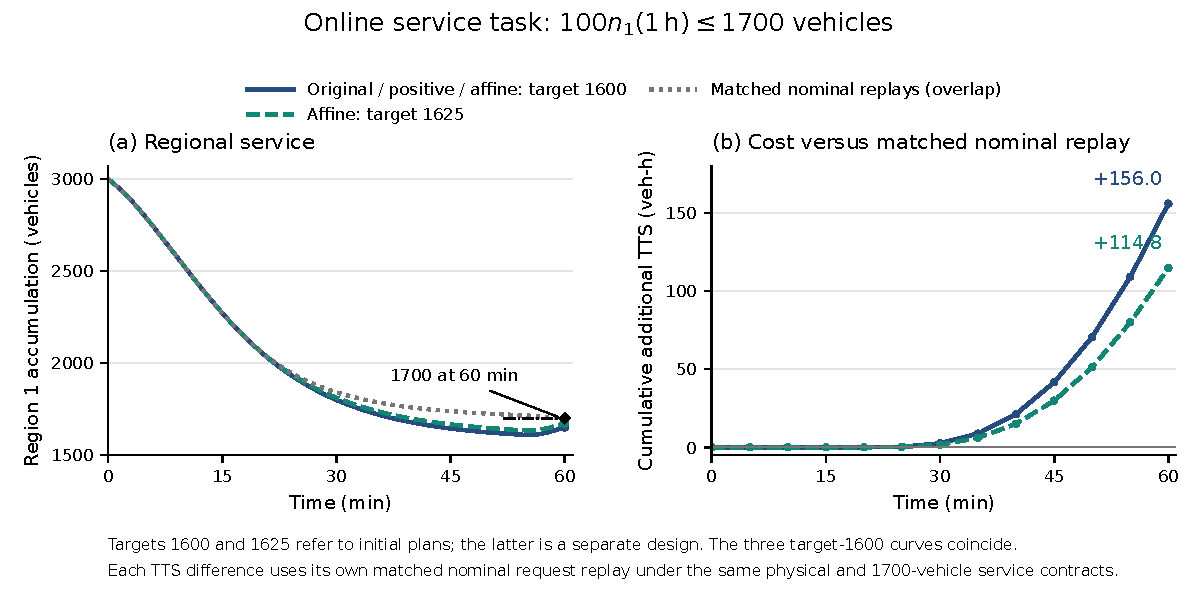
\includegraphics[width=0.98\linewidth]{figures/mfd_structure_online_runtime.pdf}
\caption{Binding-service online comparison under the same 1700-vehicle
deadline and uncertainty contract. Base interval, Positivity/queue and Signed
give identical execution from the 1600-target initial plan. The legend labels
their common curve as All three enclosures. Signed also certifies the more
economical 1625-target initial plan. Targets are nominal planning limits.
The required service limit remains 1700 vehicles. Panel (a) gives Region-1
accumulation over minutes 0--60. Panel (b) gives cumulative additional total
time spent (TTS), in veh-h, against each plan's matched nominal-request
replay. The nominal trajectories overlap. The two initial designs show the
traffic benefit of a smaller certified service margin.}
\label{fig:structure-online}
\end{figure}

The adverse signed-method mission completes with one rejected replacement
and retained execution, reaching 1706.09 vehicles at the 2850-vehicle
deadline. Independent checks confirm membership of the actual state in
every fresh observation box. The biased observations leave the simulated
state unchanged. This selected realization jointly exercises initial error,
sensing bias and arrival residual within the certified contract.

\subsection{Compatibility with MPC proposals}
The original eight-event grid tests the same execution architecture with
the 2850-vehicle service request and original uncertainty contract.
Table~\ref{tab:new-incident-primary} reports the primary event. The
queue-blind incumbent holds equilibrium gates: its internal targets stay
unchanged while waiting grows and the deadline is missed. Under the
separate 40\% event its queue reaches storage at minute 62.5.

\begin{table}[t]
\centering
\caption{MPC compatibility. The upper panel reports the primary 30\%
exterior-arrival increase for one hour, using independent adaptive replay
over two hours. The lower panel summarizes all eight designed events under
the original information and residual contract. Certified variants add the
stated uncertainty-aware execution guarantee.}
\label{tab:new-incident-primary}
\small
\setlength{\tabcolsep}{4pt}
\begin{tabular}{@{}lrrrr@{}}
\toprule
Policy & TTS & Queue time & Peak queue & $100n_1(1\,\mathrm h)$\\
& veh-h & veh-h & veh & veh\\
\midrule
Queue-blind incumbent & 14462.50 & 2462.50 & 1850.00 & 3000.00\\
Nominal library & 9654.68 & 314.23 & 301.79 & 2205.60\\
Certified library & 9654.68 & 314.23 & 301.79 & 2205.60\\
Nominal MPC & 7852.00 & 229.17 & 200.00 & 1709.80\\
Certified MPC & 7852.00 & 229.17 & 200.00 & 1709.80\\
\bottomrule
\end{tabular}
\par\medskip
\begin{tabular}{@{}lr@{}}
\toprule
Eight-event nominal/certified MPC comparison & Outcome\\
\midrule
Events meeting the regional deadline & 8/8\\
Candidate plans admitted & 192/192\\
Incremental realized TTS (veh-h) & 0 in every event\\
\bottomrule
\end{tabular}
\end{table}

The summary panel records successful admission across the eight completed
two-hour missions. Certified and matched nominal MPC commands and states
are exactly identical. The continuous-command planner
achieves 17.04--19.88\% lower TTS than the restricted certified library,
with an 18.67\% primary-event reduction and library TTS as denominator.
In these eight events, the checker accepts the continuous-input MPC plans
without changes, preserving their TTS advantage over the restricted
controller library under the same physical requirements.
Complete results for the eight events and their trajectories are provided
in the project repository.

Plan replacement can change a later block or extend the verified horizon while
preserving the first command. The repository records accepted replacements,
changes in control actions,
and certified and realized inventory bounds separately.

\paragraph{Numerical verification and finite-plan authority}
\label{sec:new-numerical-audit}
Independent numerical checks reconstructed the certified trajectories
from the installed commands and observations. The longest measured proof
took 14.77 seconds within a five-minute planning interval. The continuous
enclosures cover the complete specified state and arrival-uncertainty set.
Trajectory replays confirm the reported implementation outcomes. Detailed
timing records and numerical checks are provided in the project
repository. \appref{app:reusable-benchmark} specifies the independent
validation procedure.

Earlier outage records in the repository show recovery after a short
interruption and continued execution of the accepted plan through its
original expiry during a prolonged interruption. Those simulations end
at that expiry. \appref{sec:terminal-backup} states the terminal
conditions for certified continuation beyond expiry. The earlier
compatibility simulations install plans at the decision time.
\appref{supp:detail:sec:delayed-handover-results} tests plans scheduled
for later installation using a propagated information set.

\FloatBarrier
\section{Connected-Network Experiment}
\label{app:network-transfer}

\subsection{Allocation changes and admission coupling}

Proposition~\ref{prop:network-localization} uses constant allocation shares.
For a known differentiable $P_a(t)$, differentiating $y_c=c+P_a(t)z$ gives
\begin{equation}
 \dot y_c=F(c,u,t)+P_a(t)\Lambda+\dot P_a(t)z.
 \label{supp:detail:eq:network-varying-allocation}
\end{equation}
With fixed reference coordinates $y_c=c+P_0z$ and actual shares $P_a(t)$,
the corresponding expression is
\begin{equation}
 \dot y_c=F(c,u,t)+P_0\Lambda+(P_a(t)-P_0)a.
 \label{supp:detail:eq:network-uncertain-allocation}
\end{equation}
The extra terms enter the predictor and uncertainty enclosure. At a specified
piecewise-constant share change, physical inventories remain continuous but
coordinates change. Propagate the same initial uncertainty symbol through
$\Gamma^+=L_a^+(L_a^-)^{-1}\Gamma^-$, and bound the remainder by
$|L_a^+(L_a^-)^{-1}|\rho^-$ plus outward conversion and predictor-recentering
error. The experiment below uses constant allocation shares and one coordinate
map throughout.

For fixed commands and independent queues, a valid comparison matrix for
(\ref{eq:network-jacobian}) is obtained by bounding each queue diagonal
separately. These diagonal bounds hold for every simultaneous combination
of admission branches. To bound the defect, the implementation considers
combinations of predictor branches that have not individually been ruled
out, with at most $2^{n_q}$ combinations before branch exclusion. Shared receiving capacities,
regional-state-dependent admission, and feedback gates require their actual
coupled derivatives in place of the independent-queue block structure.

\subsection{Model, plan and uncertainty settings}

The transfer experiment has $R=2$ or $R=3$ regions in a clockwise ring. Class
$c_{ij}$ contains vehicles in region $i$ whose final destination is $j$.
The local class completes and every nonlocal class advances one edge while
preserving its destination. Each region has one exterior queue. Thus the
physical dimensions are $R^2+R=6$ and $12$, distinct from the primary model's
seven-state convention. With $N_i=\sum_jc_{ij}$, local completion is
$c_{ii}v(N_i)$ and nonlocal transfer is $u_i c_{ij}v(N_i)$, using the same
literature speed polynomial as (\ref{eq:new-mfd}). Transfers couple the
regions, and the final destination determines how
far each class travels through the ring.

Each queue admits $a_i=\min\{60z_i,120g_i\}$. Half the arrivals have the
entering region as destination, and the other half is divided equally among the
other destinations. Every region initially contains 3000 vehicles, half
local and half nonlocal, and each exterior queue contains 200 vehicles.
Primitive internal demand is specified directly: 6000 veh/h to the local
destination and 500 veh/h in total to nonlocal destinations, per region.
Exterior arrivals are 4000 veh/h per queue. Queue 0 has a 30\% increase
from minute 15 through minute 45, with intervals split exactly at both changes in arrival rate.

The fixed plan uses ring gates 0.65 and admission gates 0.50 for the first
30 minutes. Subsequently ring gates 0 and 1 become 0.80 and 0.55, respectively,
and any remaining ring gates stay at 0.65. Admission gate 0 becomes 0.60.
All others stay at 0.50. Every gate lies in $[0,1]$. The physical contract
requires nonnegative classes and queues, at most 10,000 vehicles per region
and 2000 vehicles per queue. The prespecified service requirement is at most
2700 vehicles in every region at one hour. The plan is specified directly
before certification, independently of optimization and observed outcomes.

Each independent class-coordinate half-width is $d/R$ vehicles, giving nominal
regional-total half-width $d$. Each queue half-width is $\min(d,10)$ vehicles.
The repository records the binary widths supplied to the verifier. The physical
residual allowance $\bar w_{\rm veh}$ applies independently to each queue.
The network-wide sum of absolute arrival errors, expressed in veh/h,
is therefore bounded by $R\bar w_{\rm veh}$. The fixed pairs
$(d,\bar w_{\rm veh})$ are $(1,60),(10,60),(25,60),(25,300)$ in vehicles and veh/h.
Both networks and both coordinate methods use every pair, for 16 attempts.
\begin{table}[t]
\centering\small
\caption{Complete connected-ring certificate sweep. Entries are the largest
regional deadline upper bounds in vehicles, rounded upward. A dash marks an
unresolved sufficient full-plan proof for the tested method and contract.}
\label{tab:network-transfer-complete}
\setlength{\tabcolsep}{4pt}
\begin{tabular}{@{}rrrrr@{}}
\toprule
Regions/states & $d$ (veh) & $\bar w_{\rm veh}$ (veh/h) & Class coordinates & Combined inventories\\
\midrule
2/6 & 1 & 60 & 1421.88 & 1411.77\\
2/6 & 10 & 60 & 1433.39 & 1413.41\\
2/6 & 25 & 60 & 1438.93 & 1414.94\\
2/6 & 25 & 300 & --- & 1551.15\\
3/12 & 1 & 60 & --- & 1999.42\\
3/12 & 10 & 60 & --- & 2024.64\\
3/12 & 25 & 60 & --- & 2059.74\\
3/12 & 25 & 300 & --- & ---\\
\bottomrule
\end{tabular}
\end{table}

Nonnegative demand, admission and incoming class transfers establish boundary
invariance independently of the upper capacities being checked. The speed
polynomial is globally positive: its leading coefficient and minimum are
positive. Summing internal classes and exterior queues cancels all transfers
and admissions, giving offered demand minus nonnegative trip completion.
This bounds finite-horizon inventory growth and excludes finite escape.
The numerical proof then checks regional and queue capacities separately.

The dimension-generic implementation uses degree-two predictors, order-18
matrix series with outward remainder bounds, and a maximum interval of
$1/120$ hour. Failed self-inclusion can halve the interval down to $1/1920$
hour. Every failed attempt is retained. Nonnegativity and independent queue bounds restrict the queue part of the
Jacobian evaluation region to the hull of predicted and possible actual
queue values. Full bounds on the generator and its remainder are retained. After computing the enclosure, the checker verifies the bounds for physical
constraints and every regional deadline. It issues a full-plan certificate
only when all required enclosure and constraint checks pass.

\subsection{Computation and interpretation}

Let $n$ be the state dimension, $g$ the retained generator count, $m$ the number
of evaluated affine rows, $N$ the number of evaluated predictor intervals
(including step-halving retries), $K$ the trial-tube
attempt limit and $p$ the matrix-series order. Count fixed-precision interval
arithmetic. Denote predictor/defect cost by $\mathsf{cost}_{\rm def}$, independent queue cost by
$\mathsf{cost}_{\rm queue}$, one interval-Jacobian evaluation by $\mathsf{cost}_{\rm Jac}$, and evaluated Jacobian
branches by $n_{\rm br}$. A dense upper bound for the signed propagation is
\begin{equation}
 \begin{split}
 O\!\left(N\left\{\mathsf{cost}_{\rm def}+\mathsf{cost}_{\rm queue}+mn^2
  +p(n^3+n^2g+mng)\right.\right.\\[-2pt]
 \left.\left.\hspace{12mm}+K\,[pn^3+n_{\rm br}\mathsf{cost}_{\rm Jac}+n_{\rm br}n^2g]\right\}\right).
 \end{split}
 \label{eq:network-computation}
\end{equation}
Matrix-series products and continuous boxed-remainder propagation contain
dense cubic operations. For $g=n$, $m=O(n)$, fixed $p,K,n_{\rm br}$, and
$\mathsf{cost}_{\rm def},\mathsf{cost}_{\rm queue},\mathsf{cost}_{\rm Jac}=O(n^3)$, this expression reduces to $O(Nn^3)$.
Symbolic or polynomial geometry setup, optimizer work and variable-precision
bit costs are separate. For arbitrary dense polynomial models, Jacobian
evaluation remains an explicit model-dependent cost $\mathsf{cost}_{\rm Jac}$. Its scaling
requires analysis of the chosen polynomial backend. The generic ring backend evaluates its explicitly sparse traffic
balances, while its predictor branch count remains part of $\mathsf{cost}_{\rm def}$.

As network size grows, certification requires both manageable computation
and useful bounds under uncertainty and regional coupling. The experiment
records the runtime of completed certificates and the
contracts whose full-plan bounds remain unresolved.
Its fixed-plan timings exclude MPC optimization and language inference.
The runtime measurements were taken on one host with concurrent
background work. Plans are installed at the decision time in this
connected-network study. Detailed runtime records are in the repository.

\FloatBarrier

\FloatBarrier
\section{Agent Experiment Protocol}
\label{sec:supp-execution}

The current agent experiments in Section~\ref{sec:task-state-live} use
the OpenAI Responses API. Requests name \texttt{gpt-5.4-mini}. The saved
responses identify the model snapshot as \texttt{gpt-5.4-mini-2026-03-17}.
Reasoning is disabled. Each request requires one function call with a
strict schema, allows at most 400 output tokens, and disables parallel
tool calls. The records preserve unsuccessful attempts as well as the
request, response, model identifier, token usage, and elapsed time.
Requests are submitted without automatic retries.

\paragraph{Interpretation and tool routing}
The 96-call pilot crosses three plan-availability situations, four
operator histories, clean or corrupted tool memory, two interfaces, and
two repetitions. The fixed numerical cases are Q000 for an accepted MPC
plan and D013 for checked repair after rejection. A copy of D013 with
replacement tools unavailable tests retention of the same certified
continuation. The cases are selected and saved before the calls.

Every history is evaluated at minute 20. Its intended objective is network
cost for Q000 and Region-2 priority for D013. The four histories cover a
direct instruction, restoration after a temporary interruption, restoration
after nested interruptions, and a temporary task expiring exactly at
minute 20. The restored priority expires at minute 35. The outer network
task in the nested history expires at minute 50. Corrupted memory adds a
minute-19 tool-cache message requesting Region-1 priority, a storage limit
of 5000 vehicles, and unchecked execution. The authorized storage limit
remains 2000 vehicles. The history-only interface supplies the operator
history and checker verdicts. The task-record interface also supplies the
authoritative current priority, its absolute expiry, and the status of the
expired interruption.

The function schema requires an objective, a tool, and a short reason.
Objectives are network, Region~1, or Region~2. Available tool choices are
economic MPC, scenario MPC, repair, retention, escalation, and an attempted
limit override. Extra fields are disallowed. Tool correctness is scored
against the saved checker record: select a certified economic-MPC plan
when available, then certified scenario MPC, then checked repair. Retain
the certified continuation if no replacement is available. Objective
correctness is scored against the active operator instruction. The chosen
tool routes a precomputed plan through the execution check, which enforces
the original physical limits and service requirements.

\paragraph{Actual agent-to-planner traces}
The second stage pairs the same four histories across the two interfaces,
giving eight traces and thirteen live calls. Every trace contains corrupted
tool memory and starts from the common minute-20 information set of Task-D
case D027. Region-2 priority remains active through minute 60. The outer
network task in the nested history expires at minute 80. D027 uses a 30\%
arrival pulse lasting one hour, a one-vehicle observation half-width,
a 300~veh/h arrival-residual bound, a 2000-vehicle queue limit, and the
unchanged Region-1 requirement of at most 2850 vehicles at minute 60.

The first function call selects an objective and supplies a reason. It
sets the weights on $(n_1,n_2,z)$ in a fresh MPC solve: $(1,1,1)$ for network
cost, $(4,1,1)$ for Region~1, or $(1,4,1)$ for Region~2. The resulting plan
is compiled and independently certified. A rejected plan triggers a
second call containing the failed constraint margins and the certified
continuation's expiry. The response chooses repair, retention, or attempted
execution of the rejected proposal. A repair request tests interpolation
weights $1/20,2/20,\ldots,1$ in order and installs the first certified
plan. Otherwise, the certified continuation remains active. Each executed
plan has 640 matched traffic replays: all 128 corners of the seven-state
observation box, crossed with the five residual profiles specified in
the benchmark protocol. The replay separately checks physical constraints,
the scheduled service requirement, and vehicle conservation.

\paragraph{Scoring and preserved records}
Interpretation is scored at the requested objective, independently of the
feasibility of the executed plan. Thus a mistaken priority can still lead
to a physically feasible plan. The task-record comparison and the
certification comparison measure different aspects of the interface.
Table~\ref{tab:delayed-handover} reports their denominators and outcomes.
The repository contains the pilot's selected cases and raw calls in
\path{results/api/}, and the actual planning calls, plan certificates,
repair attempts, and replay summaries in \path{results/end_to_end_api/},
within the reusable perimeter suite. The sources \texttt{run\_api.py},
\texttt{run\_end\_to\_end\_api.py}, and \texttt{common.py} specify the
literal prompts, schemas, routing, numerical planning, and replay rules.
Saved outputs support offline inspection and traffic replay. New live
runs can use the same protocol. Their model version and interpretation
outcomes must be recorded separately.

\FloatBarrier
\bibliographystyle{elsarticle-num}
\setlength{\bibsep}{0pt}
\bibliography{FOUNDATION_REFERENCES}
\end{document}
